%!TEX root = Manuscript.tex

\chapter{Result of precise matching}
\label{chap:appendixB}
\zll{In Section \ref{Comparisonof6variantsP}, we demonstrate the matches visualization and \ac{DoD}s of precise matching results on representative datasets Fr{\'e}jus and Alberona. In this section the remaining results on other datasets (i.e., Pezenas and Kobe) are displayed.}
%In this section we demonstrate the matches visualizations and \ac{DoD}s of precise matching results on datasets Pezenas and Kobe.\\
\section{Matches visualization}
\label{sec:PrecisematchViz}
For both datasets, there exist 2 epochs, leading to 1 set of epoch combination for precise matching. Four variants (i.e., \ding{172} $Patch_{SpGDSM}$, \ding{173} $Guided_{SpGDSM}$, \ding{174} $Patch_{SIFTDSM}$ and \ding{175} $Guided_{SIFTDSM}$) are tested on both datasets, the resulted matches are visualized in Figure \ref{MatchVizPezenas} and \ref{MatchVizKobe}. 
%For each dataset, every possible combination of 2 epochs are matched with 4 variants (\ding{172} $Patch_{SpGDSM}$, \ding{173} $Guided_{SpGDSM}$, \ding{174} $Patch_{SIFTDSM}$ and \ding{175} $Guided_{SIFTDSM}$). 
%\begin{enumerate}
%	\item For Pezenas, there exist 2 epochs, leading to 1 set of epoch combination, the matches visualization of which is displayed in Figure \ref{MatchVizPezenas}.
%	\item For Kobe, there exist 2 epochs, leading to 1 set of epoch combination, the matches visualization of which is displayed in Figure \ref{MatchVizKobe}.
%\end{enumerate}
As can be seen, patterns similar to Fr{\'e}jus and Alberona (c.f., Section \ref{para:DiscussionP}) are present.% in Pezenas and Kobe. %:\\
%Patterns similar to Fr{\'e}jus and Alberona (elaborated in Section \ref{matchVizMainBody}) are present in Pezenas and Kobe. %:\\
%\begin{enumerate}
%	\item $Patch$ recovered considerably more matches than $Guided$, which is understandable as SuperGlue is more invariant over time than SIFT.\\
%	\item 3D-RANSAC filter and cross correlation removed considerable number of matches, yet enough matches survived.
%\end{enumerate}


%%%%%%%%%%%%%%%%%Pezenas
\begin{figure*}[htbp]
	\begin{center}
		\subfigure[Overlapping zone]{
			\begin{minipage}[t]{0.48\linewidth}
				\centering
				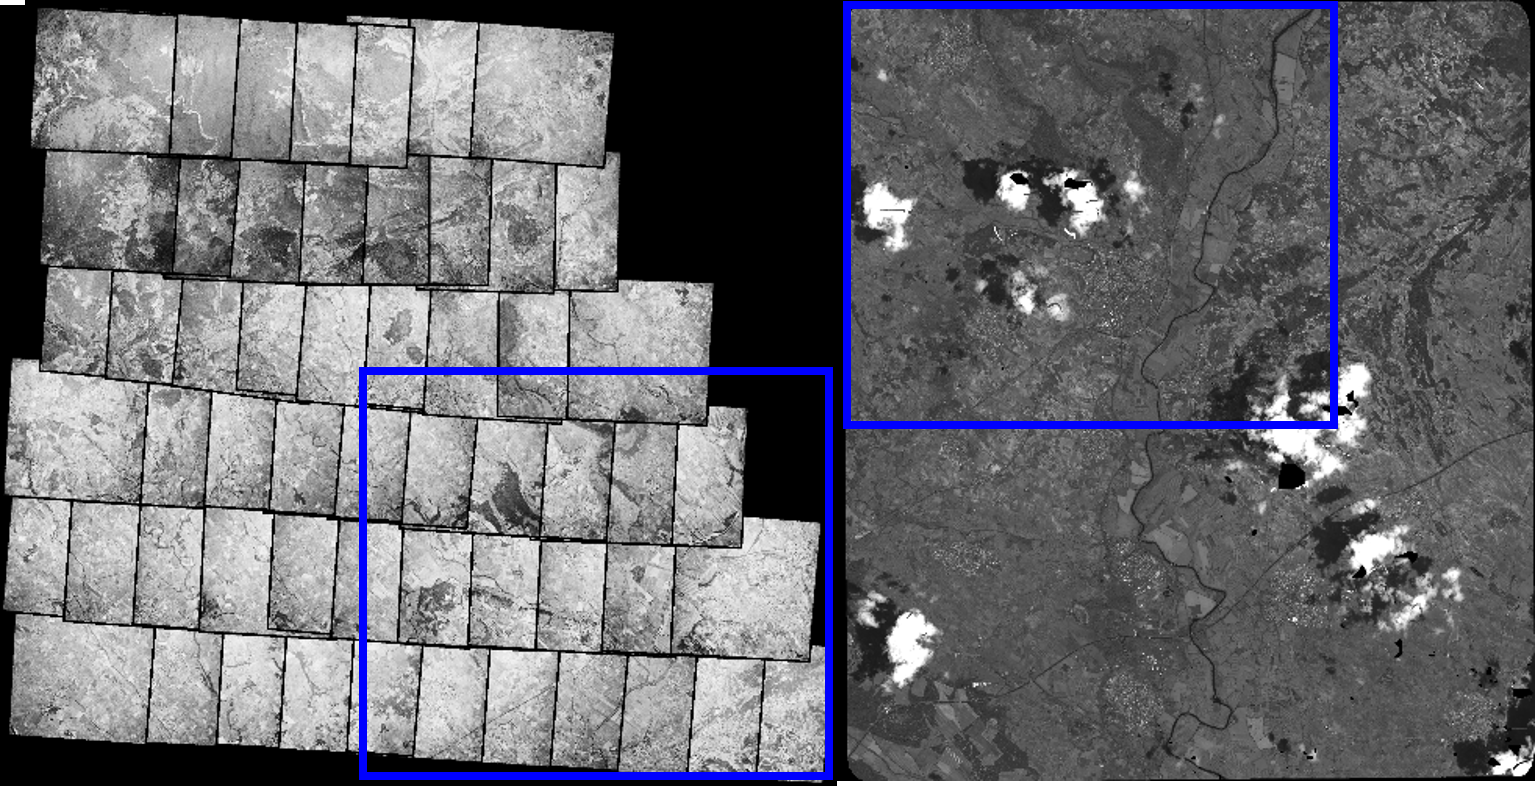
\includegraphics[width=6.8cm]{images/Chapitre4/Pseudo-Ortho-MEC-Malt_Tapas_1971_Ortho-MEC-Malt_Satellite.png}
			\end{minipage}%
		}
		\subfigure[Number of recovered matches]{
			\begin{minipage}[t]{0.48\linewidth}
				\centering
				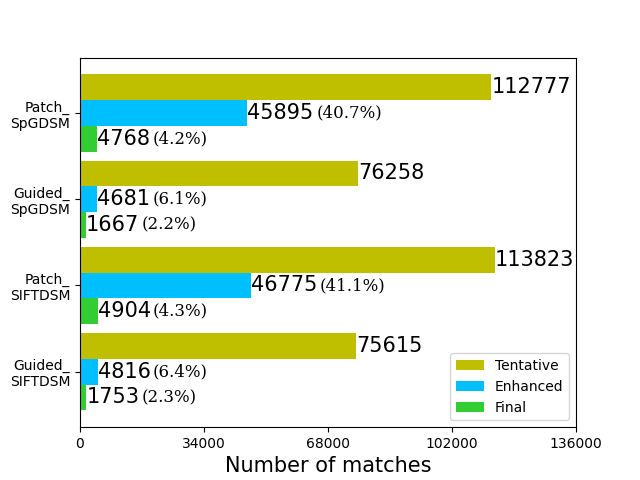
\includegraphics[width=5.8cm]{images/Chapitre4/PlotBarH-Pezenas1971-2014.png}
			\end{minipage}%
		}
		\subfigure[$Patch_{SpGDSM}$]{
			\begin{minipage}[t]{0.48\linewidth}
				\centering
				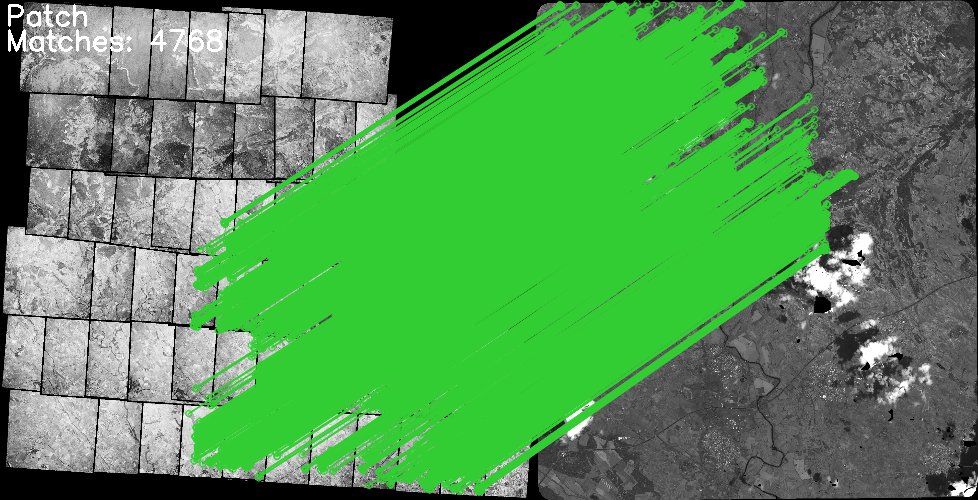
\includegraphics[width=6.8cm]{images/Chapitre4/Precise-SpGDSMHomol-SuperGlue-3DRANSAC-CrossCorrelation-PileImg_Ortho-MEC-Malt_Tapas_1971_Ortho-MEC-Malt_Satellite.png}
			\end{minipage}%
		}
		\subfigure[$Guided_{SpGDSM}$]{
			\begin{minipage}[t]{0.48\linewidth}
				\centering
				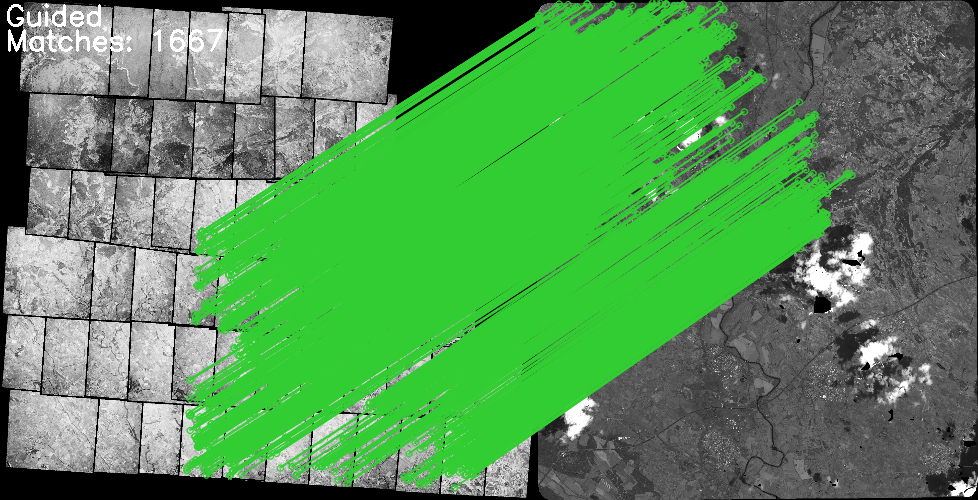
\includegraphics[width=6.8cm]{images/Chapitre4/Precise-SpGDSMHomol-GuidedSIFT-3DRANSAC-CrossCorrelation-PileImg_Ortho-MEC-Malt_Tapas_1971_Ortho-MEC-Malt_Satellite.png}
			\end{minipage}%
		}
		\subfigure[$Patch_{SIFTDSM}$]{
			\begin{minipage}[t]{0.48\linewidth}
				\centering
				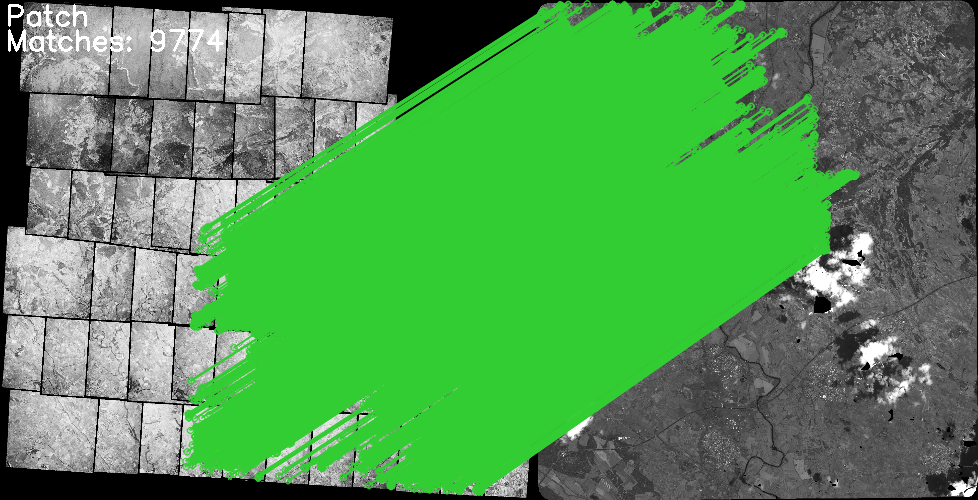
\includegraphics[width=6.8cm]{images/Chapitre4/Precise-SIFTDSMHomol-SuperGlue-3DRANSAC-CrossCorrelation-PileImg_Ortho-MEC-Malt_Tapas_1971_Ortho-MEC-Malt_Satellite.png}
			\end{minipage}%
		}
		\subfigure[$Guided_{SIFTDSM}$]{
			\begin{minipage}[t]{0.48\linewidth}
				\centering
				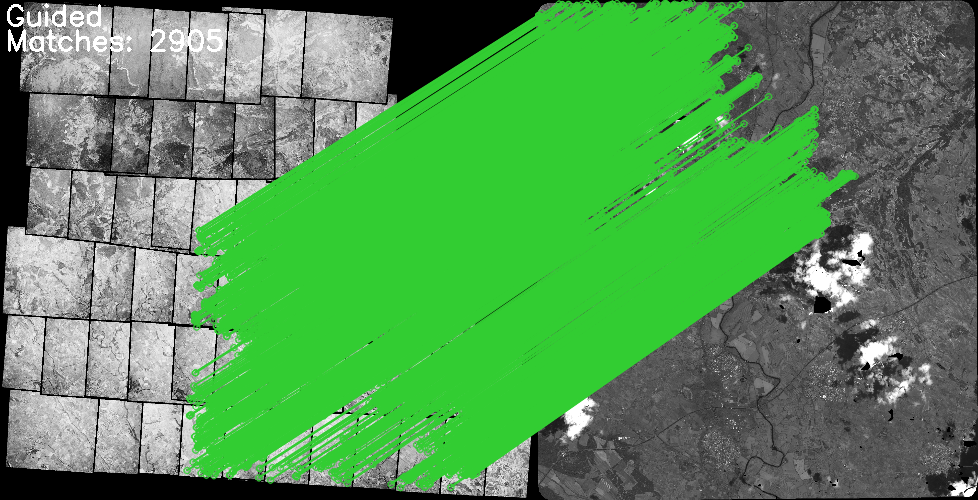
\includegraphics[width=6.8cm]{images/Chapitre4/Precise-SIFTDSMHomol-GuidedSIFT-3DRANSAC-CrossCorrelation-PileImg_Ortho-MEC-Malt_Tapas_1971_Ortho-MEC-Malt_Satellite.png}
			\end{minipage}%
		}
		\caption{Precise matching visualization of \textbf{Pezenas 1971 and 2014 (Satellite)}. (a) Image pairs to be matched, with red rectangles indicating the overlapping zone. (b) Numbers of tentative, enhanced and final matches recovered with $Patch_{SpGDSM}$, $Guided_{SpGDSM}$, $Patch_{SIFTDSM}$ and $Guided_{SIFTDSM}$ individually. (c-f) Visualization of final matches recovered with $Patch_{SpGDSM}$, $Guided_{SpGDSM}$, $Patch_{SIFTDSM}$ and $Guided_{SIFTDSM}$ individually.}
		\label{MatchVizPezenas}
	\end{center}
\end{figure*} 

%Pseudo-Ortho-MEC-Malt_Tapas_1991_Ortho-MEC-Malt_Tapas_1994

\begin{figure*}[htbp]
	\begin{center}
		\subfigure[Overlapping zone]{
			\begin{minipage}[t]{0.48\linewidth}
				\centering
				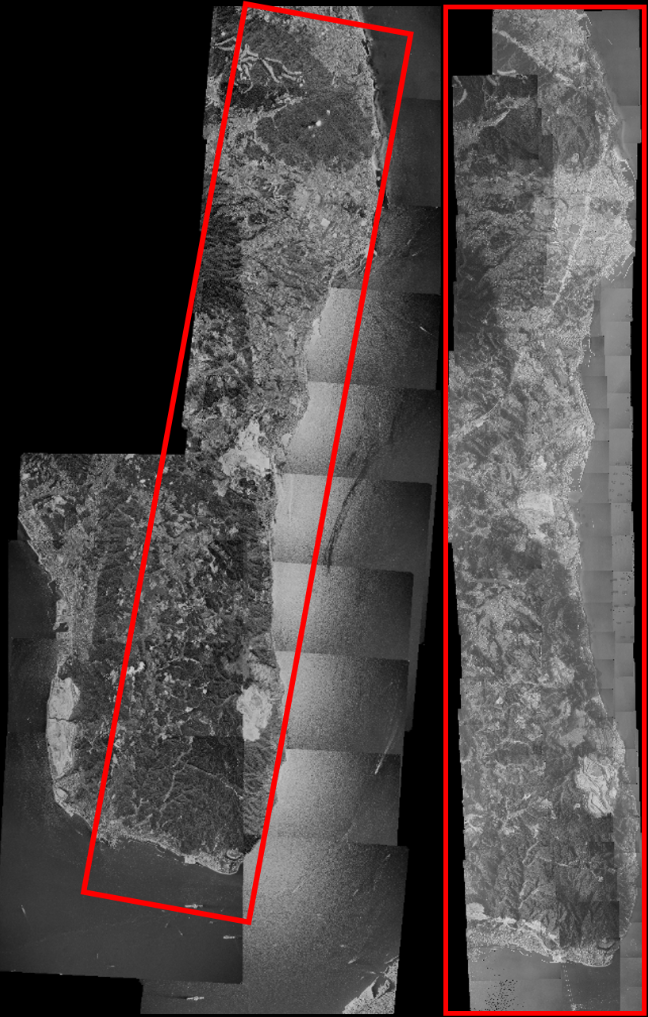
\includegraphics[width=3.8cm,angle=90]{images/Chapitre3/Pseudo-Ortho-MEC-Malt_Tapas_1991_Ortho-MEC-Malt_Tapas_1994.png}
			\end{minipage}%
		}
		\subfigure[Number of recovered matches]{
			\begin{minipage}[t]{0.48\linewidth}
				\centering
				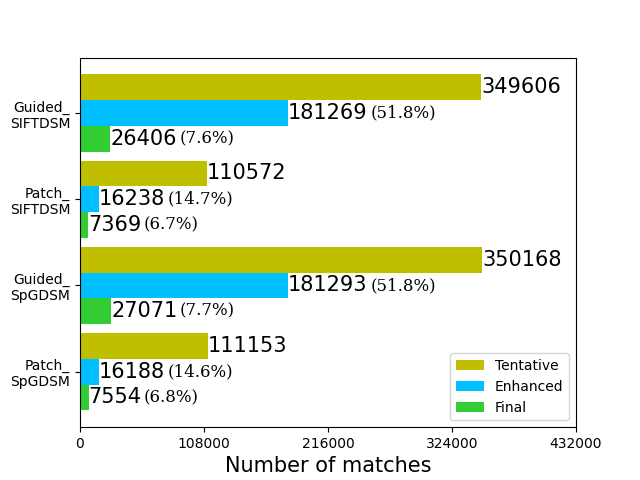
\includegraphics[width=5.8cm]{images/Chapitre4/PlotBarH-Kobe1991-1995.png}
			\end{minipage}%
		}
		\subfigure[$Patch_{SpGDSM}$]{
			\begin{minipage}[t]{0.48\linewidth}
				\centering
				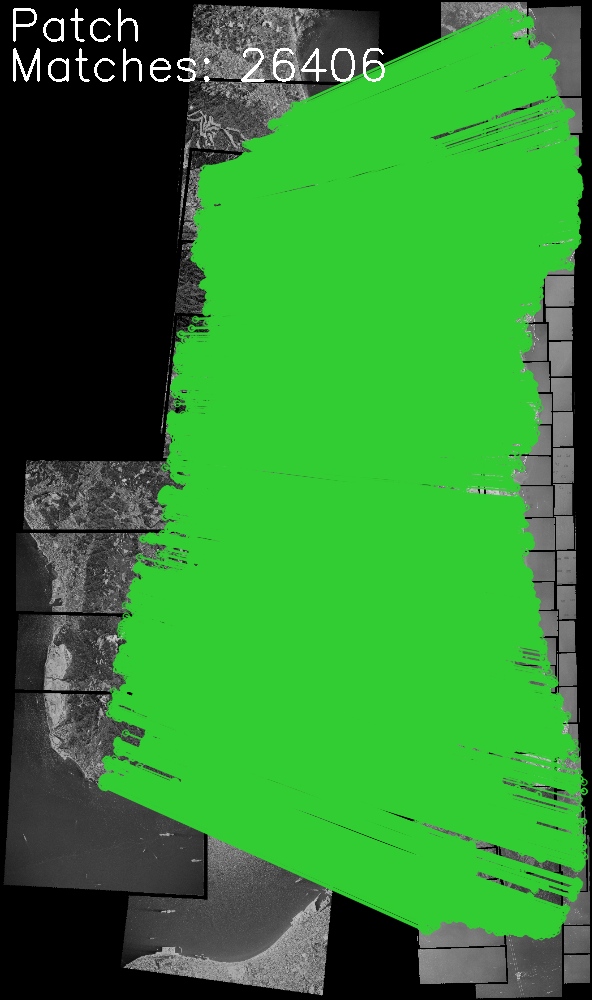
\includegraphics[width=3.8cm,angle=90]{images/Chapitre4/Precise-SpGDSMHomol-SuperGlue-3DRANSAC-CrossCorrelation-PileImg_Ortho-MEC-Malt_Tapas_1991_Ortho-MEC-Malt_Tapas_1994.png}
			\end{minipage}%
		}
		\subfigure[$Guided_{SpGDSM}$]{
			\begin{minipage}[t]{0.48\linewidth}
				\centering
				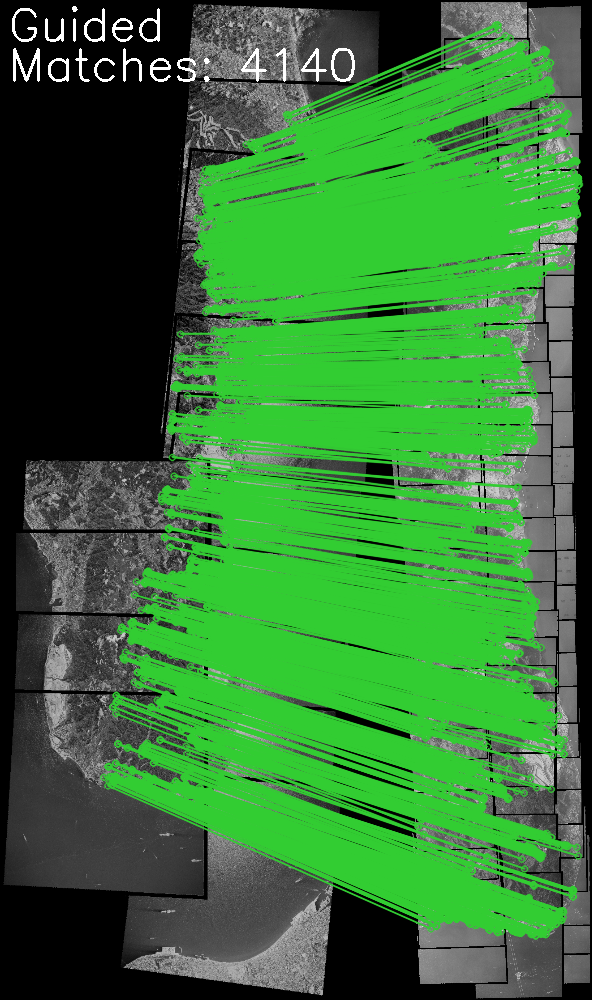
\includegraphics[width=3.8cm,angle=90]{images/Chapitre4/Precise-SpGDSMHomol-GuidedSIFT-3DRANSAC-CrossCorrelation-PileImg_Ortho-MEC-Malt_Tapas_1991_Ortho-MEC-Malt_Tapas_1994.png}
			\end{minipage}%
		}
		\subfigure[$Patch_{SIFTDSM}$]{
			\begin{minipage}[t]{0.48\linewidth}
				\centering
				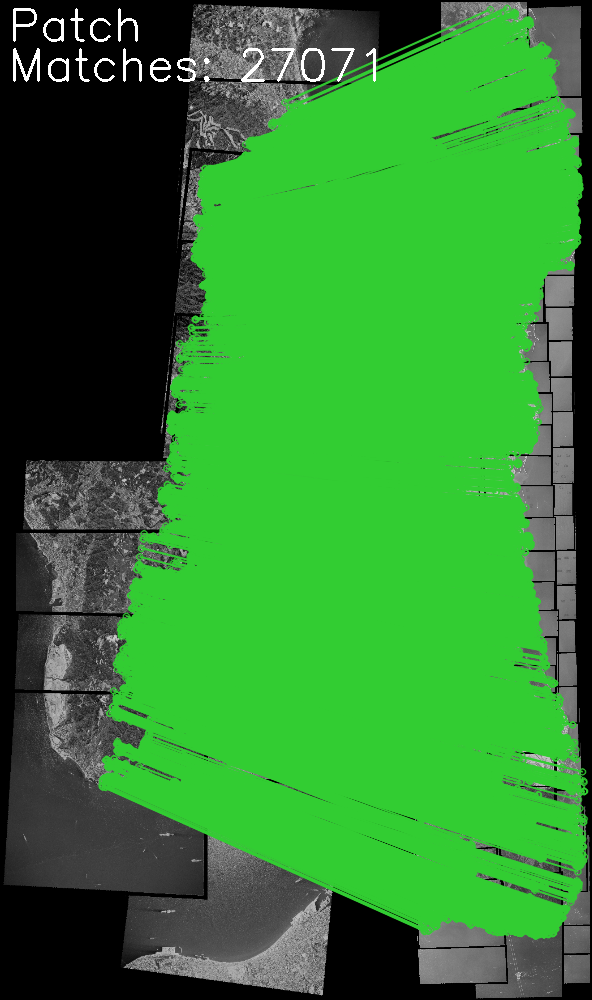
\includegraphics[width=3.8cm,angle=90]{images/Chapitre4/Precise-SIFTDSMHomol-SuperGlue-3DRANSAC-CrossCorrelation-PileImg_Ortho-MEC-Malt_Tapas_1991_Ortho-MEC-Malt_Tapas_1994.png}
			\end{minipage}%
		}
		\subfigure[$Guided_{SIFTDSM}$]{
			\begin{minipage}[t]{0.48\linewidth}
				\centering
				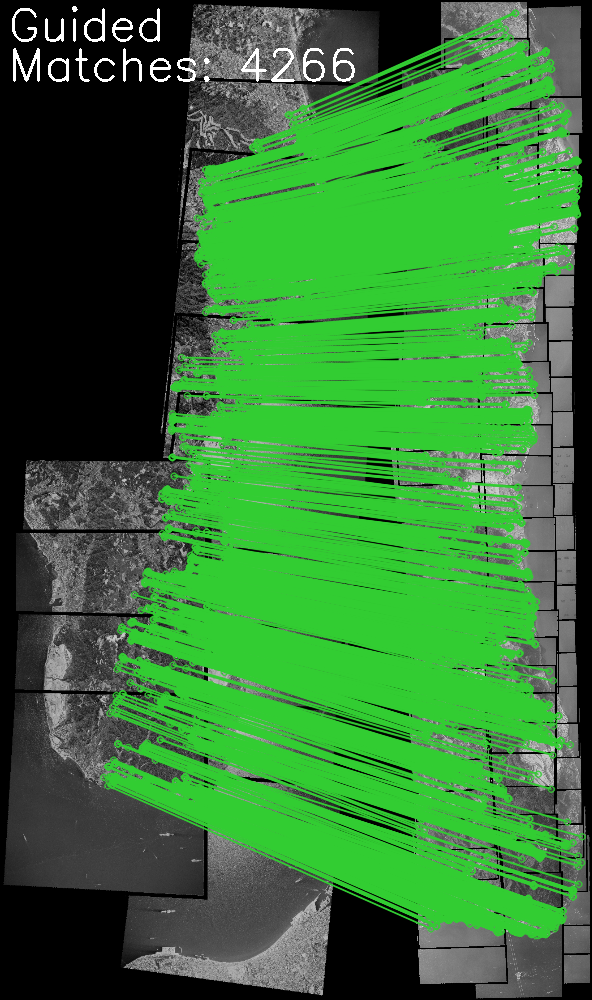
\includegraphics[width=3.8cm,angle=90]{images/Chapitre4/Precise-SIFTDSMHomol-GuidedSIFT-3DRANSAC-CrossCorrelation-PileImg_Ortho-MEC-Malt_Tapas_1991_Ortho-MEC-Malt_Tapas_1994.png}
			\end{minipage}%
		}
		\caption{Precise matching visualization of \textbf{Kobe 1991 and 1995}. (a) Image pairs to be matched, with red rectangles indicating the overlapping zone. (b) Numbers of tentative, enhanced and final matches recovered with $Patch_{SpGDSM}$, $Guided_{SpGDSM}$, $Patch_{SIFTDSM}$ and $Guided_{SIFTDSM}$ individually. (c-f) Visualization of final matches recovered with $Patch_{SpGDSM}$, $Guided_{SpGDSM}$, $Patch_{SIFTDSM}$ and $Guided_{SIFTDSM}$ individually.}
		\label{MatchVizKobe}
	\end{center}
\end{figure*} 

\section{DoD}
\label{sec:PreciseDoD}
The \ac{DoD}s for Pezenas and Kobe are demonstrated in Figure~\ref{PreciseDoDPezenas-Satellite} and ~\ref{PreciseDoDKobe}. 
%In each figure, the \ac{DoD}s resulted from rough co-registered orientations using variants $SuperGlue_{DSM}$ and $SIFT_{DSM}$ (elaborated in Chapter~\ref{chap:RoughCoReg}, hereinafter referred to as DoD$^{SpGDSM}$ and DoD$^{SIFTDSM}$) are displayed as bases, and the \ac{DoD}s resulted from refined orientations using variants $Patch_{SpGDSM}$, $Guided_{SpGDSM}$, $Patch_{SIFTDSM}$ and $Guided_{SIFTDSM}$ (hereinafter termed as DoD$^{Patch_{SpGDSM}}$, DoD$^{Guided_{SpGDSM}}$, DoD$^Patch_{SIFTDSM}$ and DoD$^Guided_{SIFTDSM}$) are given for comparison. 
The corresponding statistical information is displayed in Table~\ref{PreciseDoDStatistic1}.
As can be seen, patterns similar to Fr{\'e}jus and Alberona (c.f., Section \ref{para:DiscussionP}) are present.% in Pezenas and Kobe. %:\\

%For both datasets, the \textit{dome} effect presented in DoD$^{SpGDSM}$ and DoD$^{SIFTDSM}$ (the first column of the subgraphs) is mitigated in DoD$^{Patch_{SpGDSM}}$, DoD$^{Guided_{SpGDSM}}$, DoD$^Patch_{SIFTDSM}$ and DoD$^Guided_{SIFTDSM}$ (the second and third column of subgraphs). 
%According to the absolute average value $|\mu|$ of all the \ac{DoD}s in Figure \ref{PreciseDoDPezenas-Satellite} and \ref{PreciseDoDKobe} (cf. Talbe \ref{PreciseDoDStatistic1}), $Guided$ leads to \ac{DoD}s with slightly better accuracy than $Patch$.\\

\begin{figure*}[htbp]
	\begin{center}
		\subfigure[\ac{DoD}$_{Pezenas1971}^{{SpGDSM}}$]{
			\begin{minipage}[t]{0.31\linewidth}
				\centering
				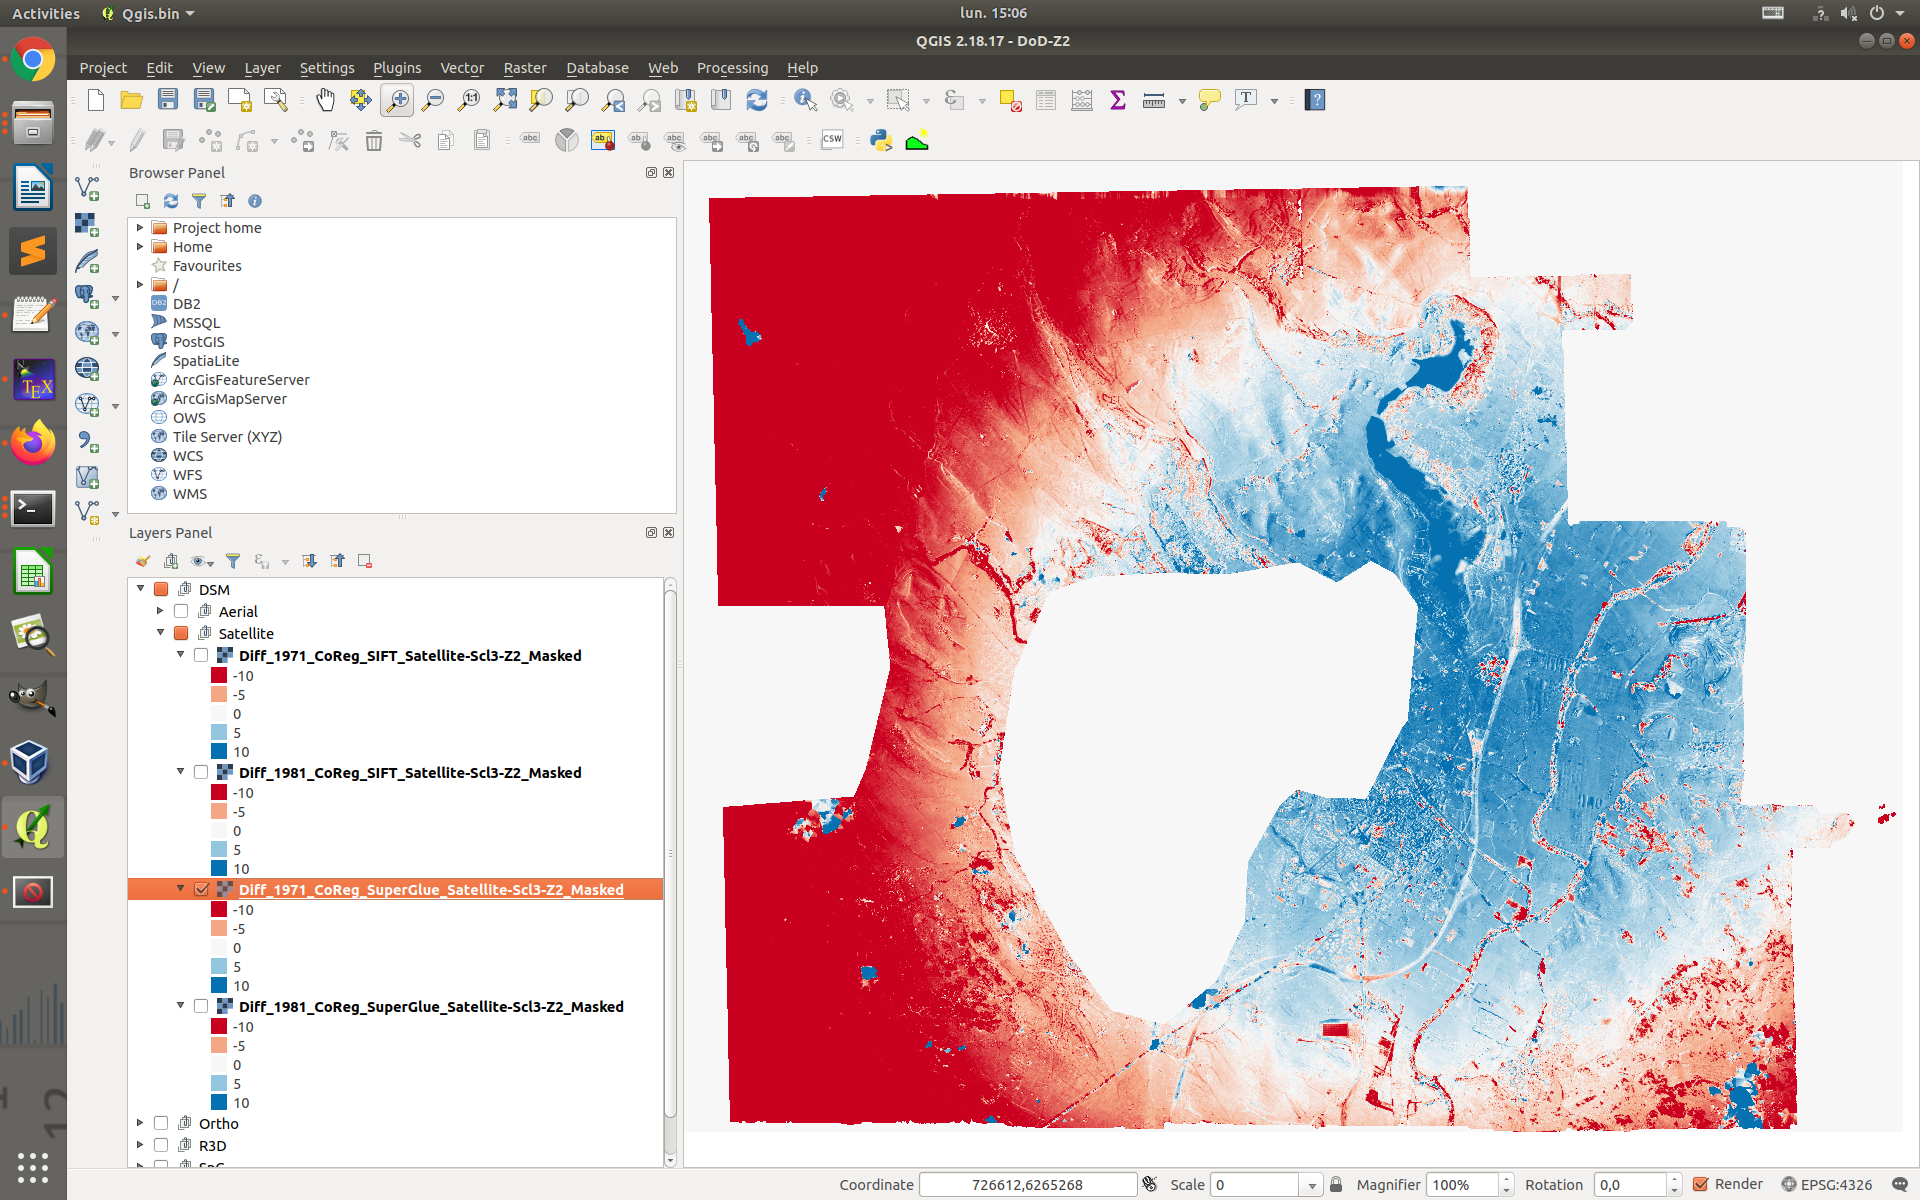
\includegraphics[width=4.5cm,trim=740 80 50 230,clip]{images/Chapitre3/DoD1971DSM-SuperGlue-Satellite.png}
			\end{minipage}%
		}
		\subfigure[\ac{DoD}$_{Pezenas1971}^{Patch_{SpGDSM}}$]{
			\begin{minipage}[t]{0.31\linewidth}
				\centering
				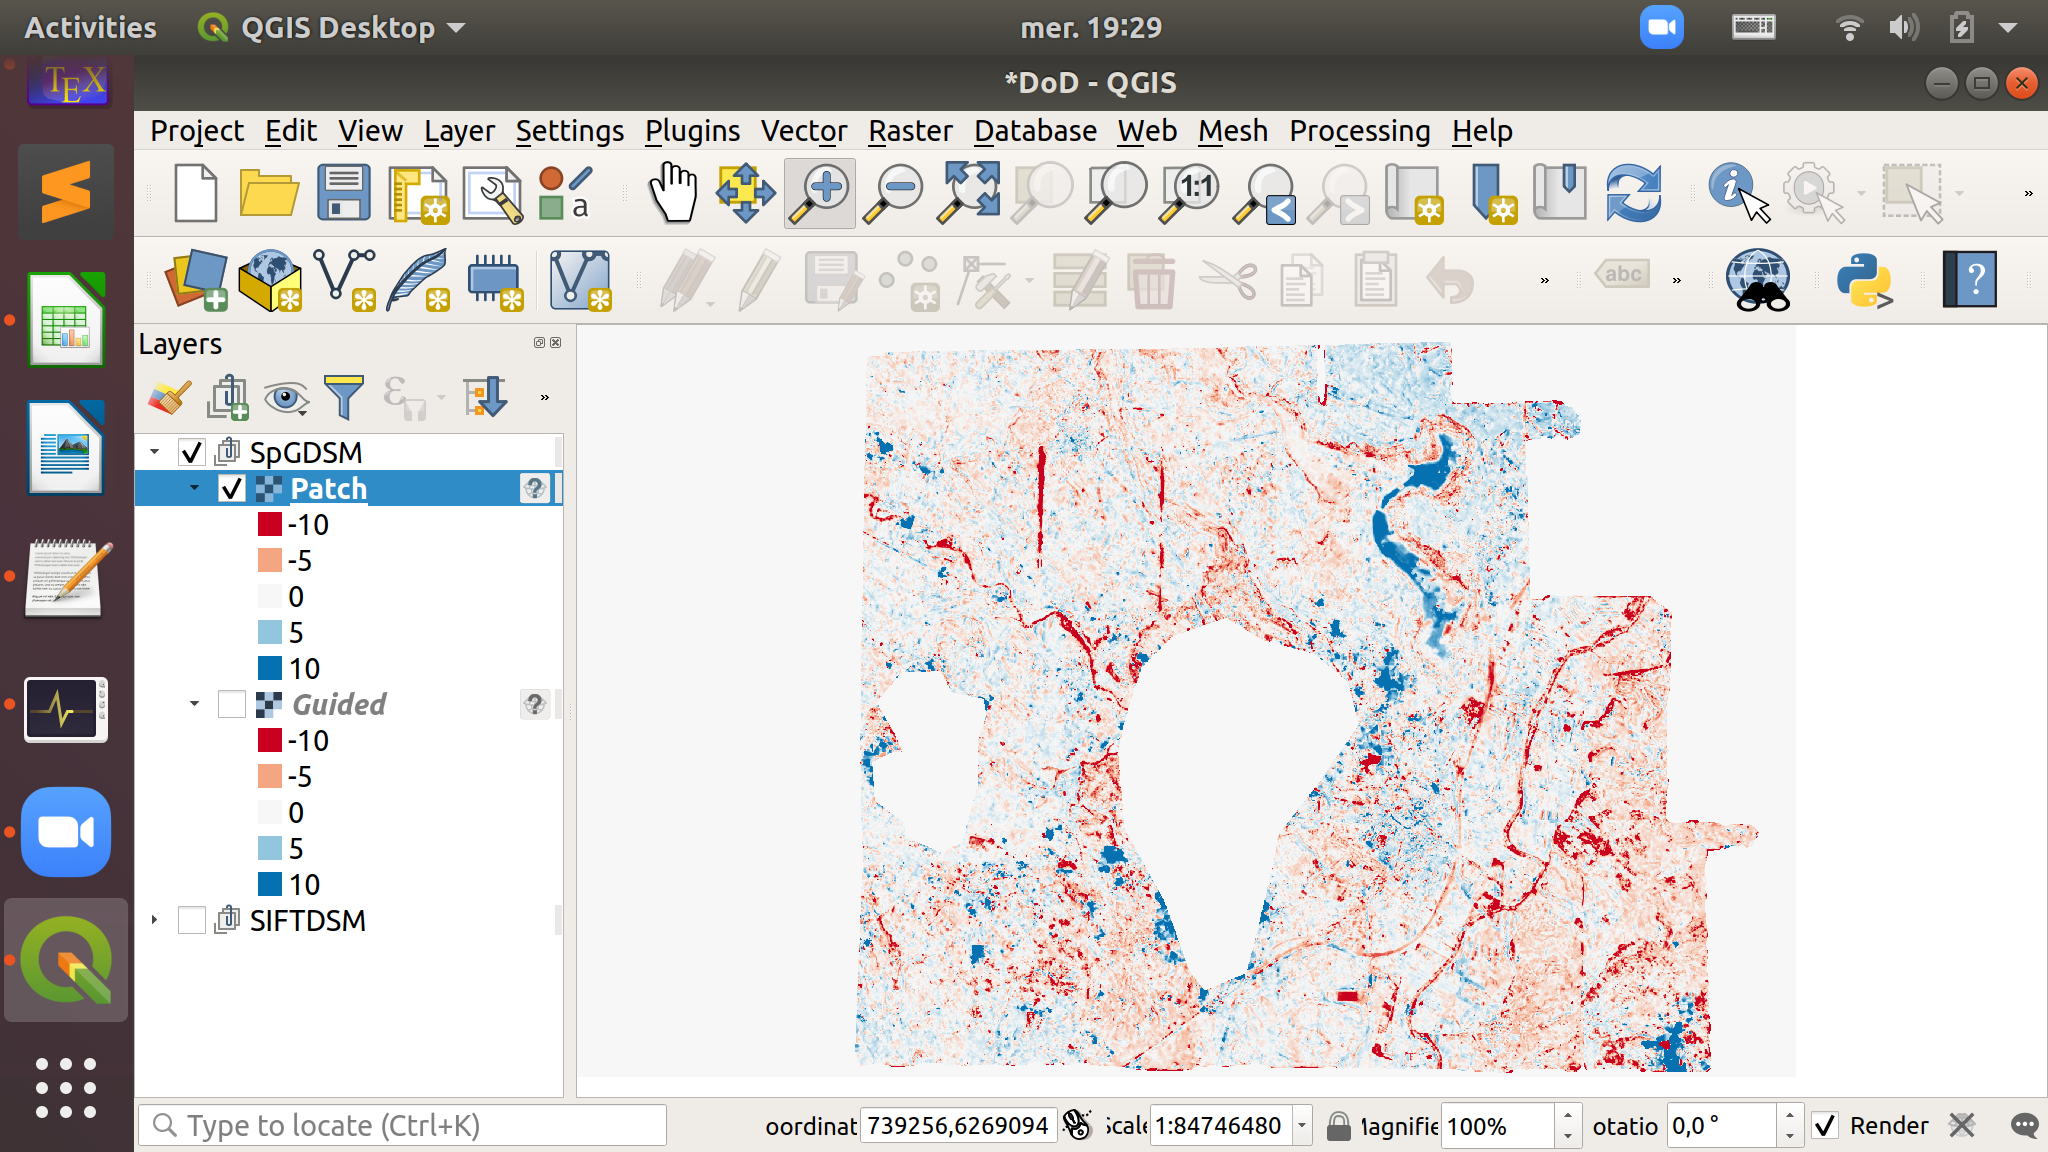
\includegraphics[width=4.5cm,trim=840 70 290 340,clip]{images/Chapitre4/DoD1971_Patch_SpGDSM.png}
			\end{minipage}%
		}
		\subfigure[\ac{DoD}$_{Pezenas1971}^{Guided_{SpGDSM}}$]{
			\begin{minipage}[t]{0.31\linewidth}
				\centering
				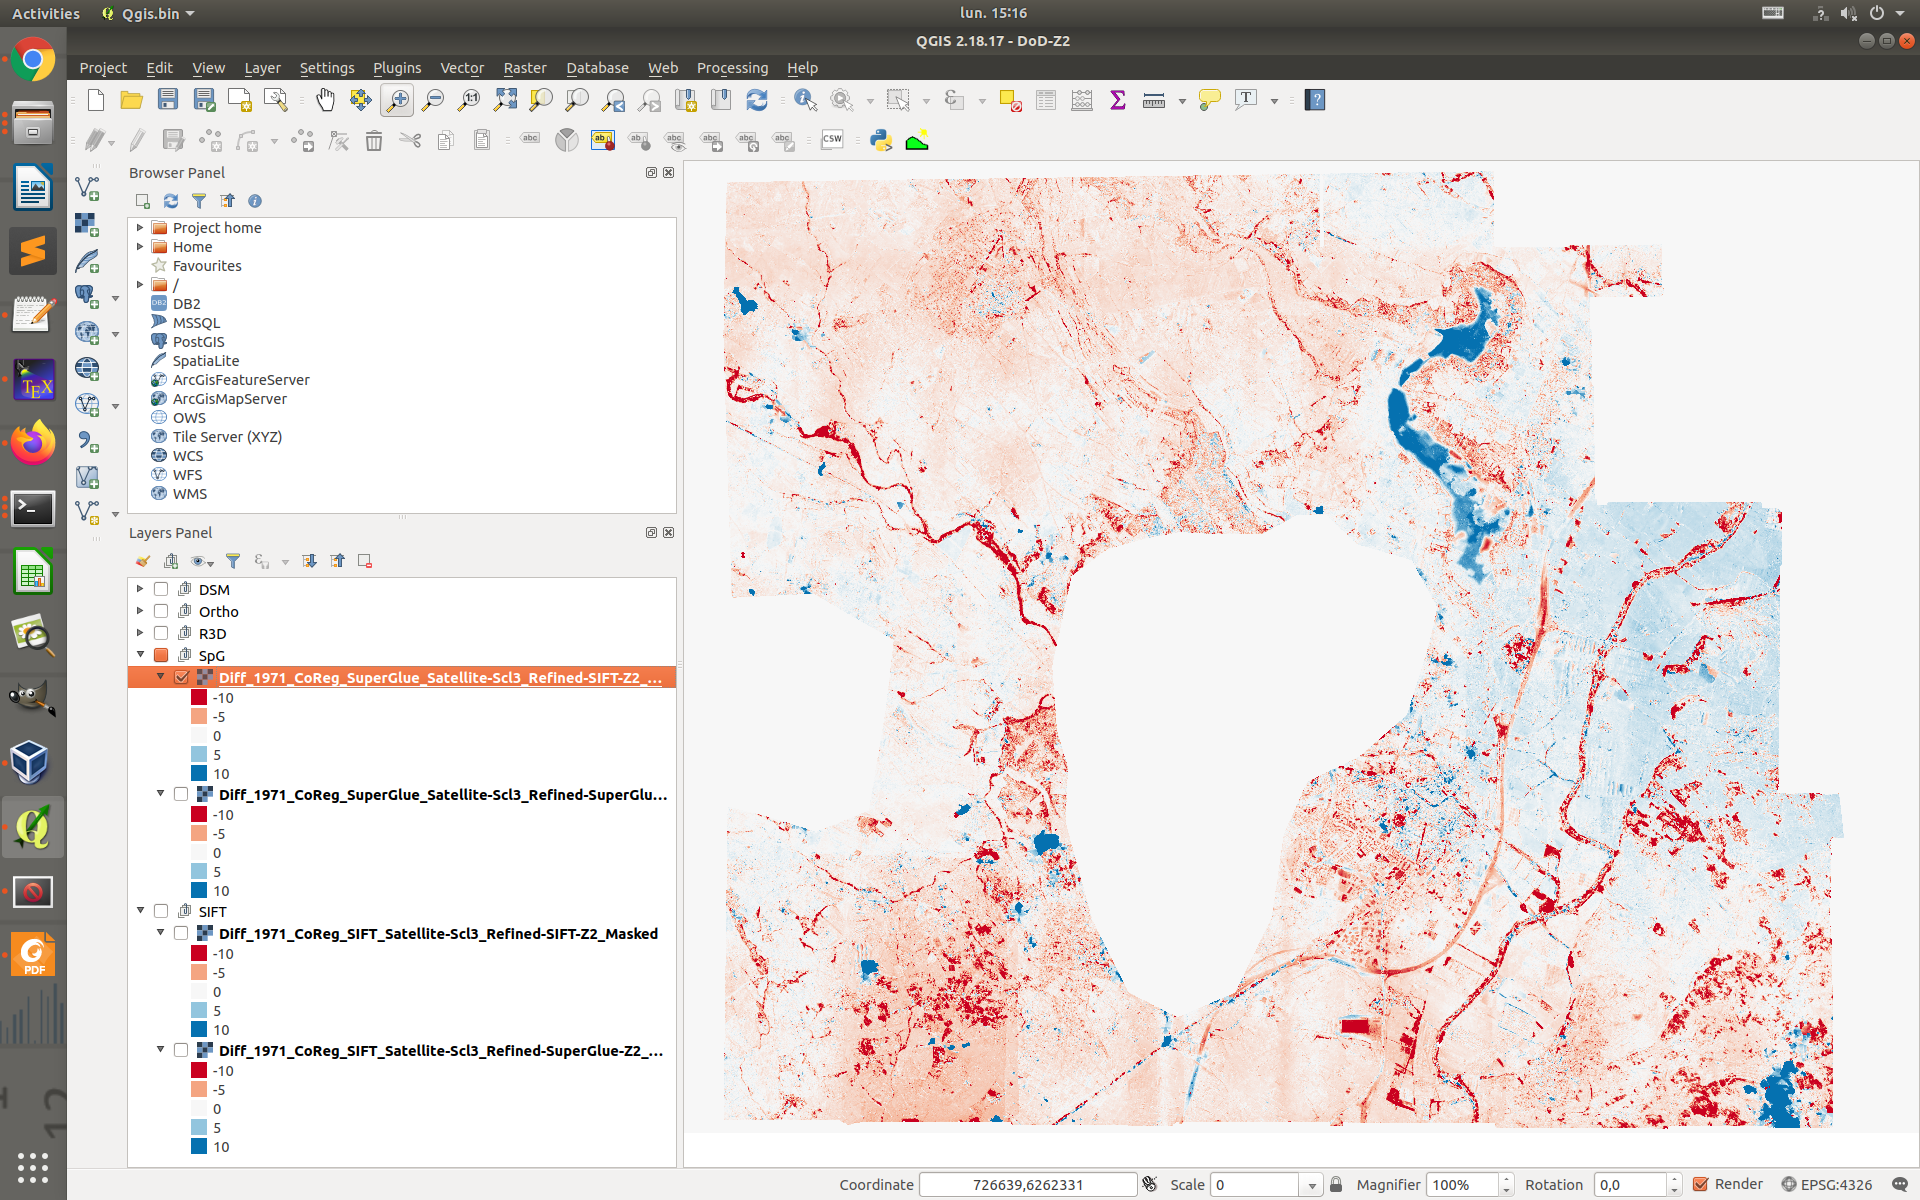
\includegraphics[width=4.5cm,trim=840 70 290 340,clip]{images/Chapitre4/DoD1971_Guided_SpGDSM.png}
			\end{minipage}%
		}\\
		\subfigure[\ac{DoD}$_{Pezenas1971}^{{SIFTDSM}}$]{
			\begin{minipage}[t]{0.31\linewidth}
				\centering
				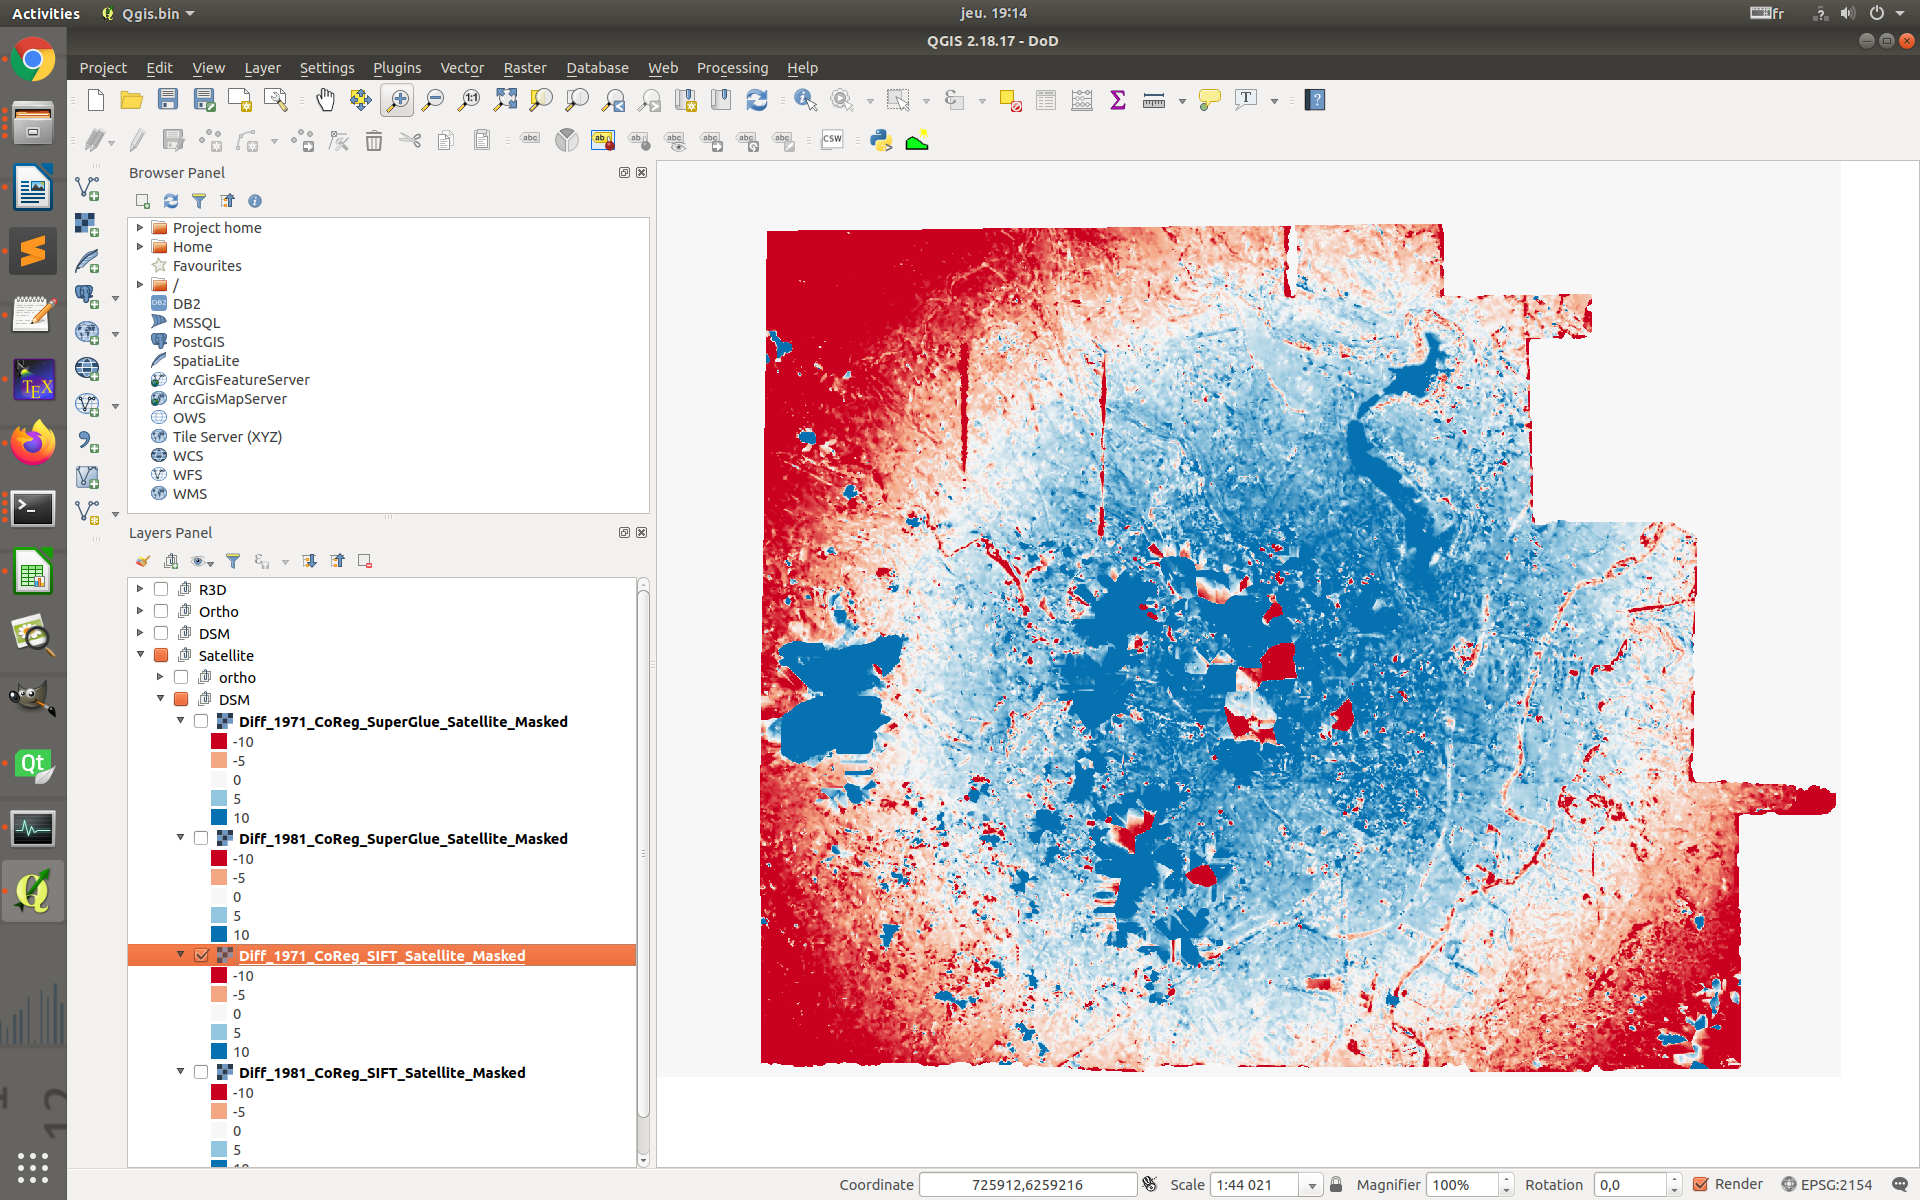
\includegraphics[width=4.5cm,trim=740 100 50 200,clip]{images/Chapitre3/DoD1971DSM-SIFT-Satellite.png}
			\end{minipage}%
		}
		\subfigure[\ac{DoD}$_{Pezenas1971}^{Patch_{SIFTDSM}}$]{
			\begin{minipage}[t]{0.31\linewidth}
				\centering
				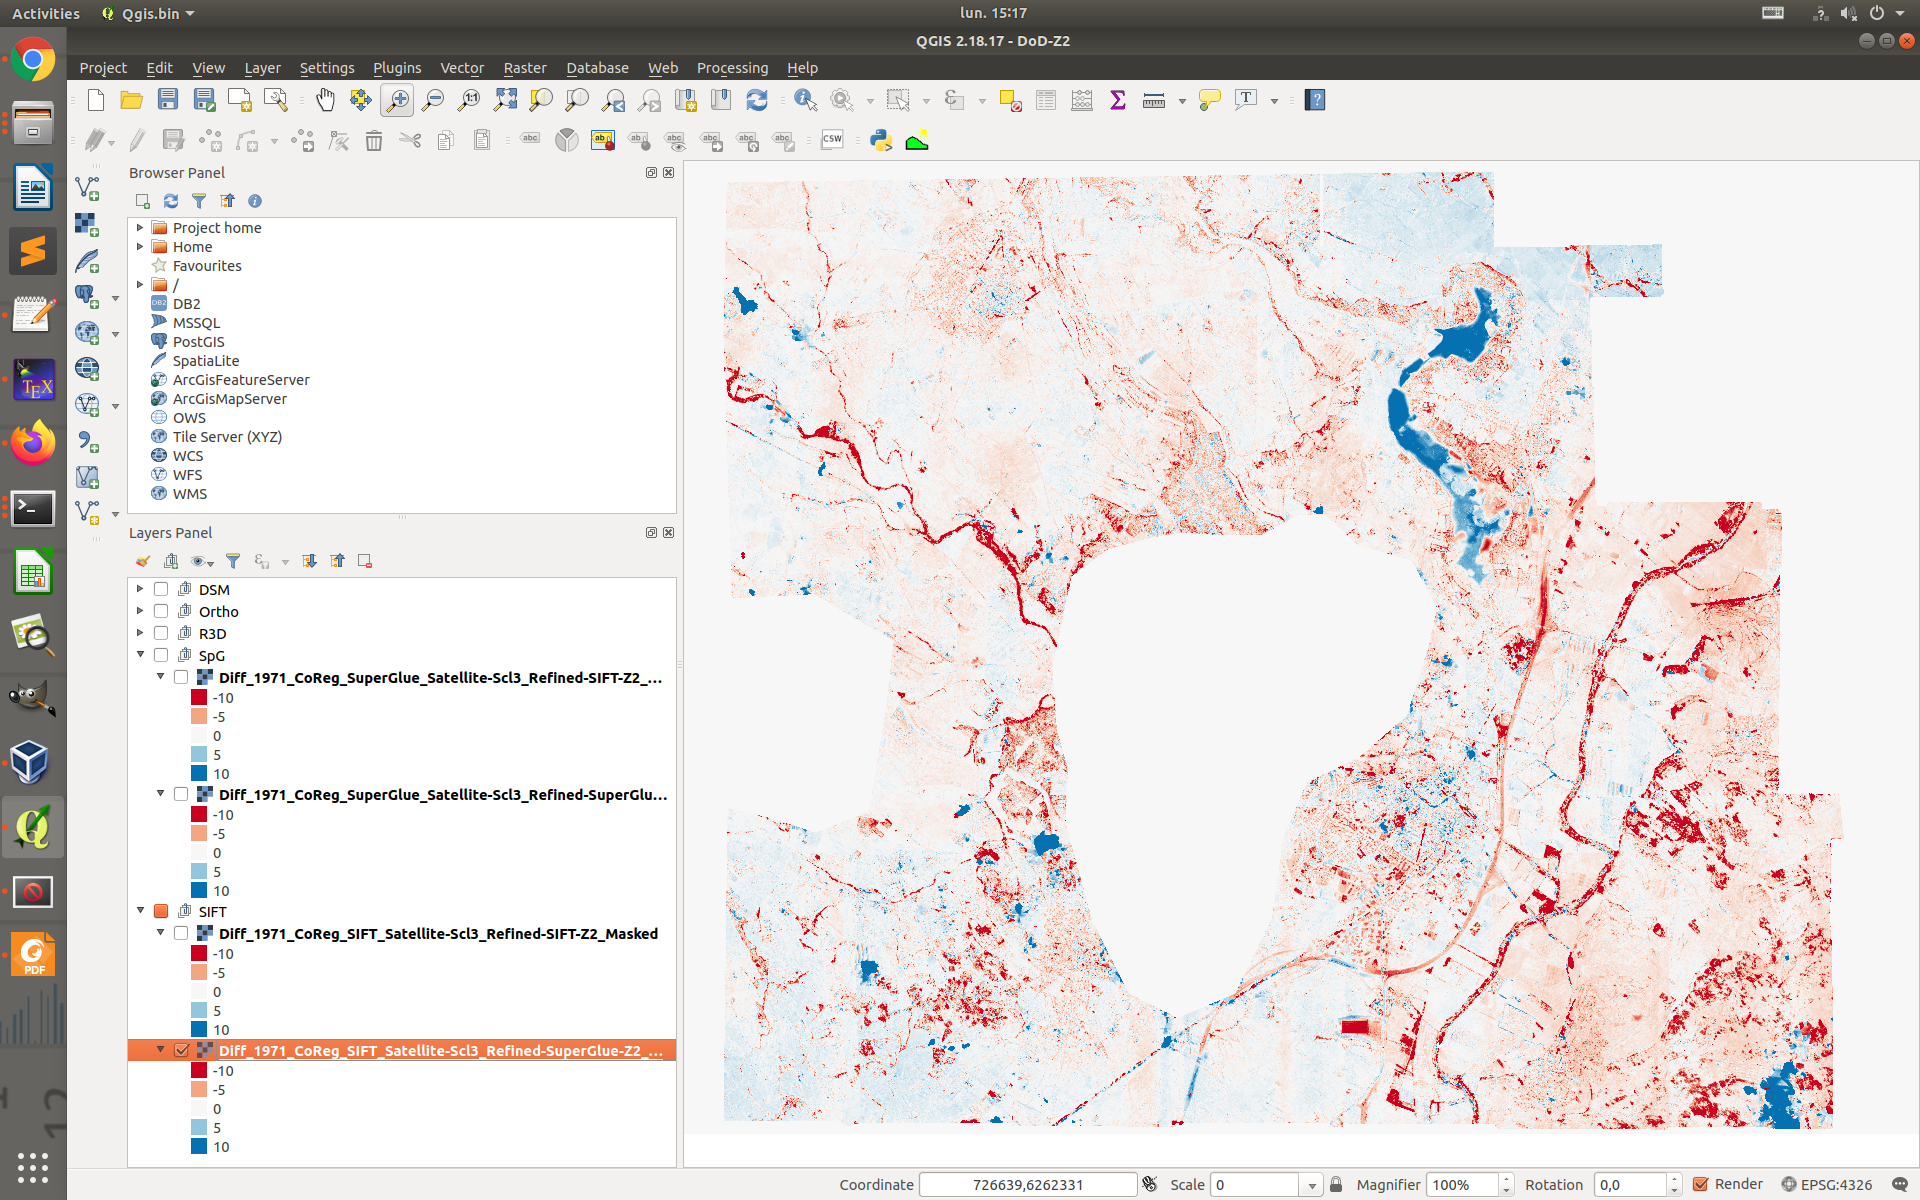
\includegraphics[width=4.5cm,trim=840 70 290 340,clip]{images/Chapitre4/DoD1971_Patch_SIFTDSM.png}
			\end{minipage}%
		}
		\subfigure[\ac{DoD}$_{Pezenas1971}^{Guided_{SIFTDSM}}$]{
			\begin{minipage}[t]{0.31\linewidth}
				\centering
				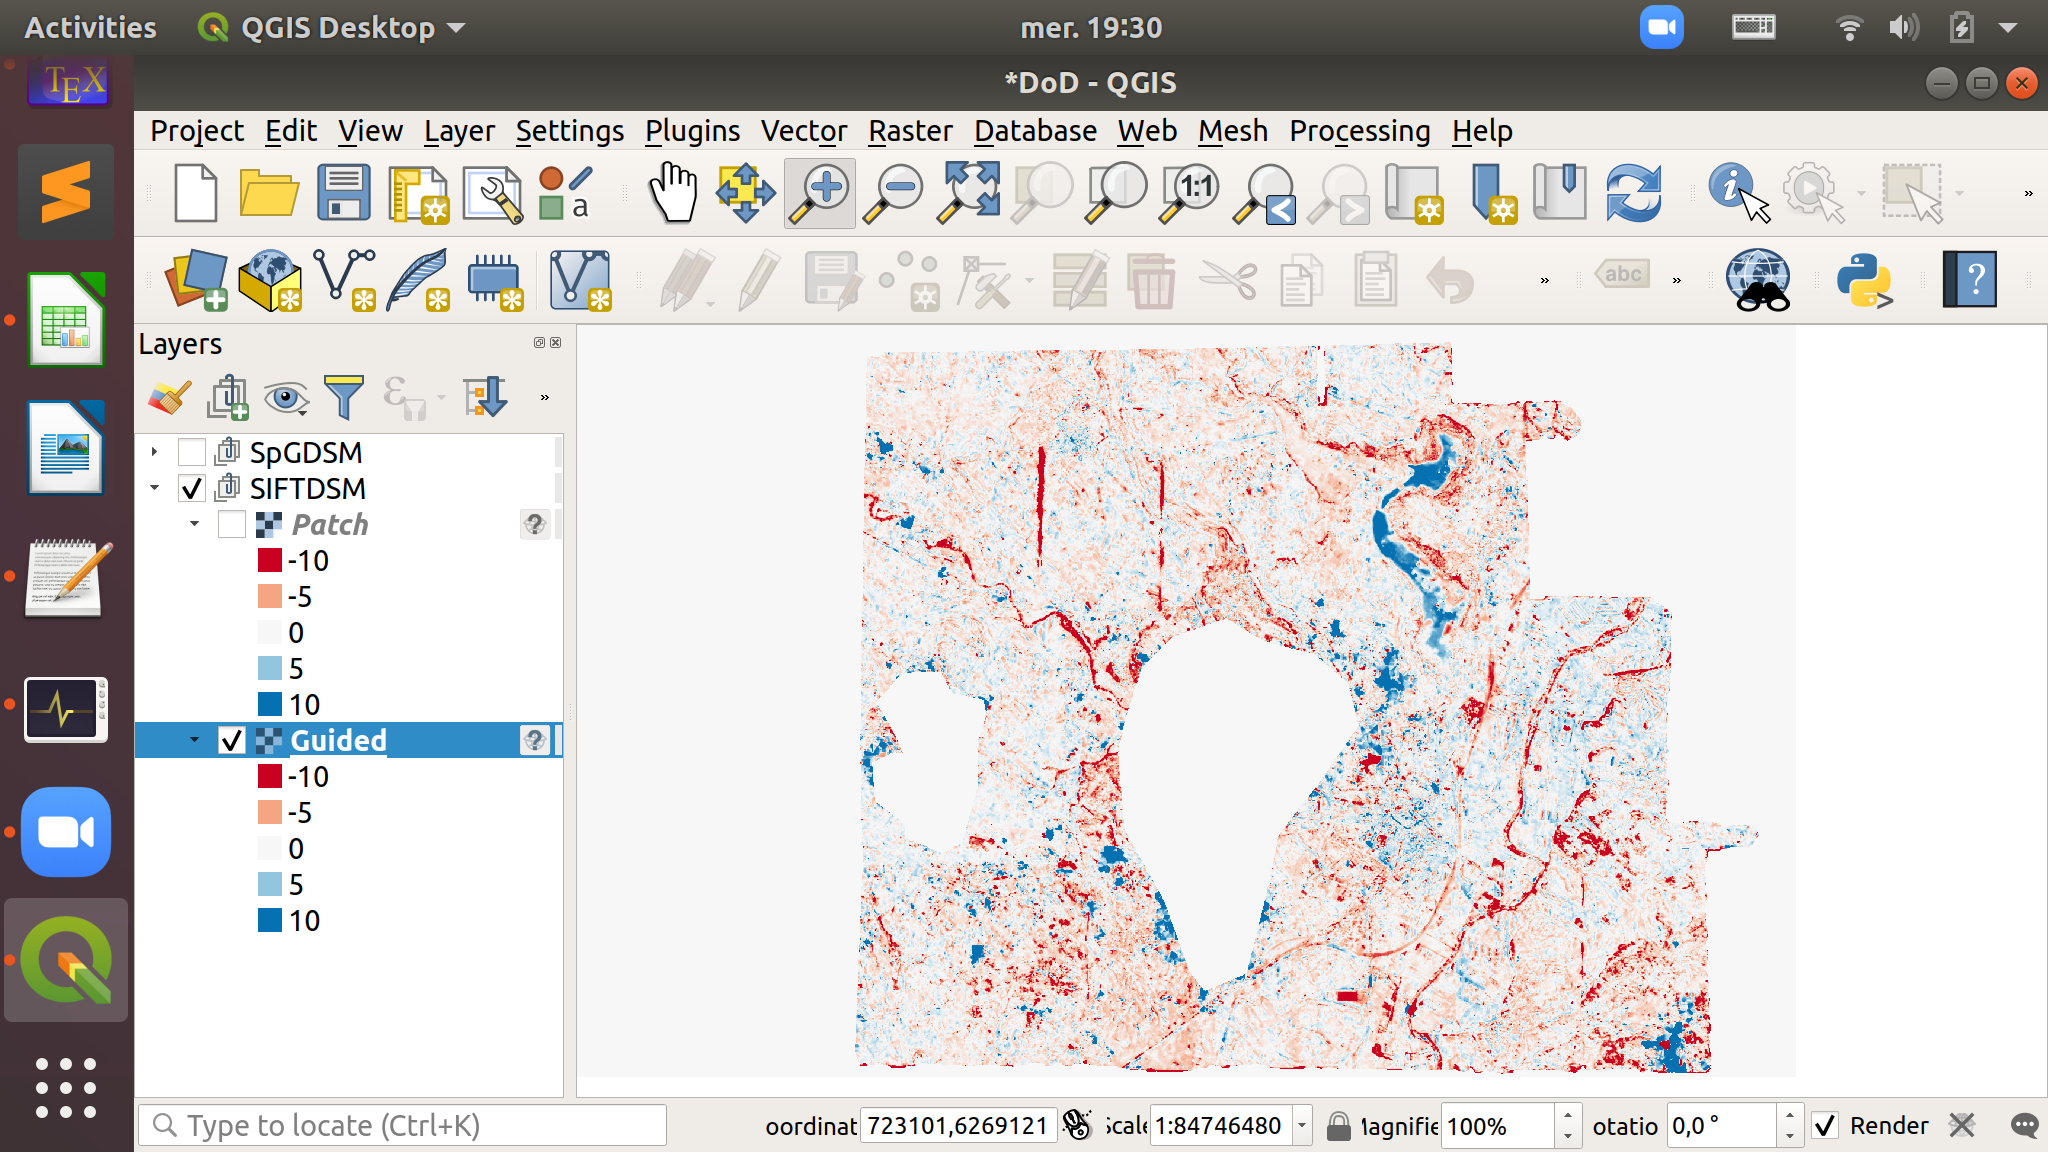
\includegraphics[width=4.5cm,trim=840 70 290 340,clip]{images/Chapitre4/DoD1971_Guided_SIFTDSM.png}
			\end{minipage}%
		}\\
		
		\subfigure[\ac{DoD} legend]{
			\begin{minipage}[t]{1\linewidth}
				\centering
				
\includegraphics[width=11cm]{images/Chapitre4/LegendDoD.png}
			\end{minipage}%
		}
		\caption{{\ac{DoD}s between free epoch \textbf{Pezenas 1971} and reference satellite epoch \textbf{2014}. (a) and (d) are roughly co-registered \ac{DoD}s resulted from variants $SuperGlue_{DSM}$ and $SIFT_{DSM}$ (elaborated in Chapter \ref{chap:RoughCoReg}). (b, c, e, f) are refined \ac{DoD}s resulted from variants $Patch_{SpGDSM}$, $Guided_{SpGDSM}$, $Patch_{SIFTDSM}$ and $Guided_{SIFTDSM}$ individually. The holes among them are areas covered with clouds which are masked out.}}
		\label{PreciseDoDPezenas-Satellite}
	\end{center}
\end{figure*} 


\begin{figure*}[htbp]
	\begin{center}
		\subfigure[\ac{DoD}$_{Kobe}^{{SpGDSM}}$]{
			\begin{minipage}[t]{1\linewidth}
				\centering
				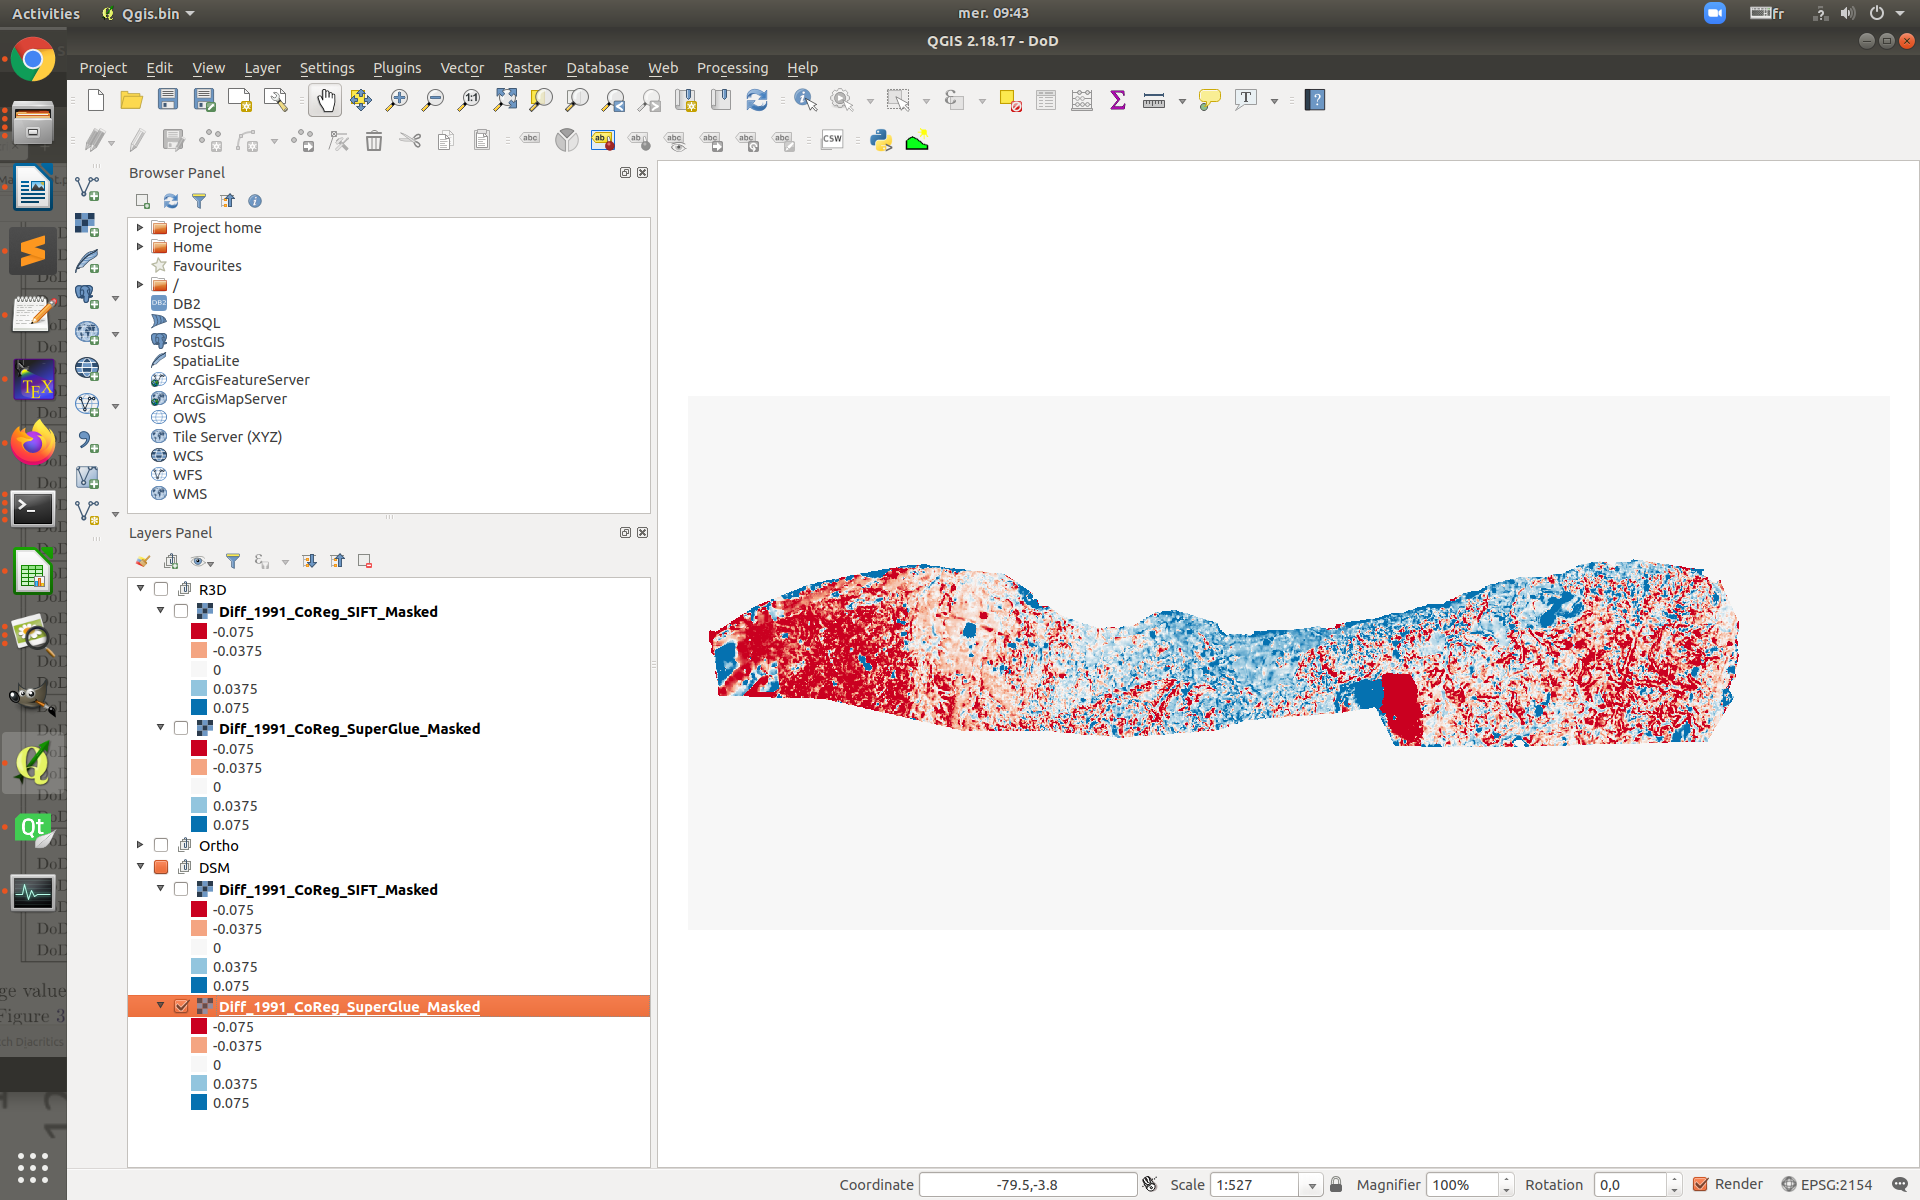
\includegraphics[width=12cm,trim=700 450 180 560,clip]{images/Chapitre3/DoD1991DSM-SuperGlue.png}
			\end{minipage}%
		}
		\subfigure[\ac{DoD}$_{Kobe}^{Patch_{SpGDSM}}$]{
			\begin{minipage}[t]{1\linewidth}
				\centering
				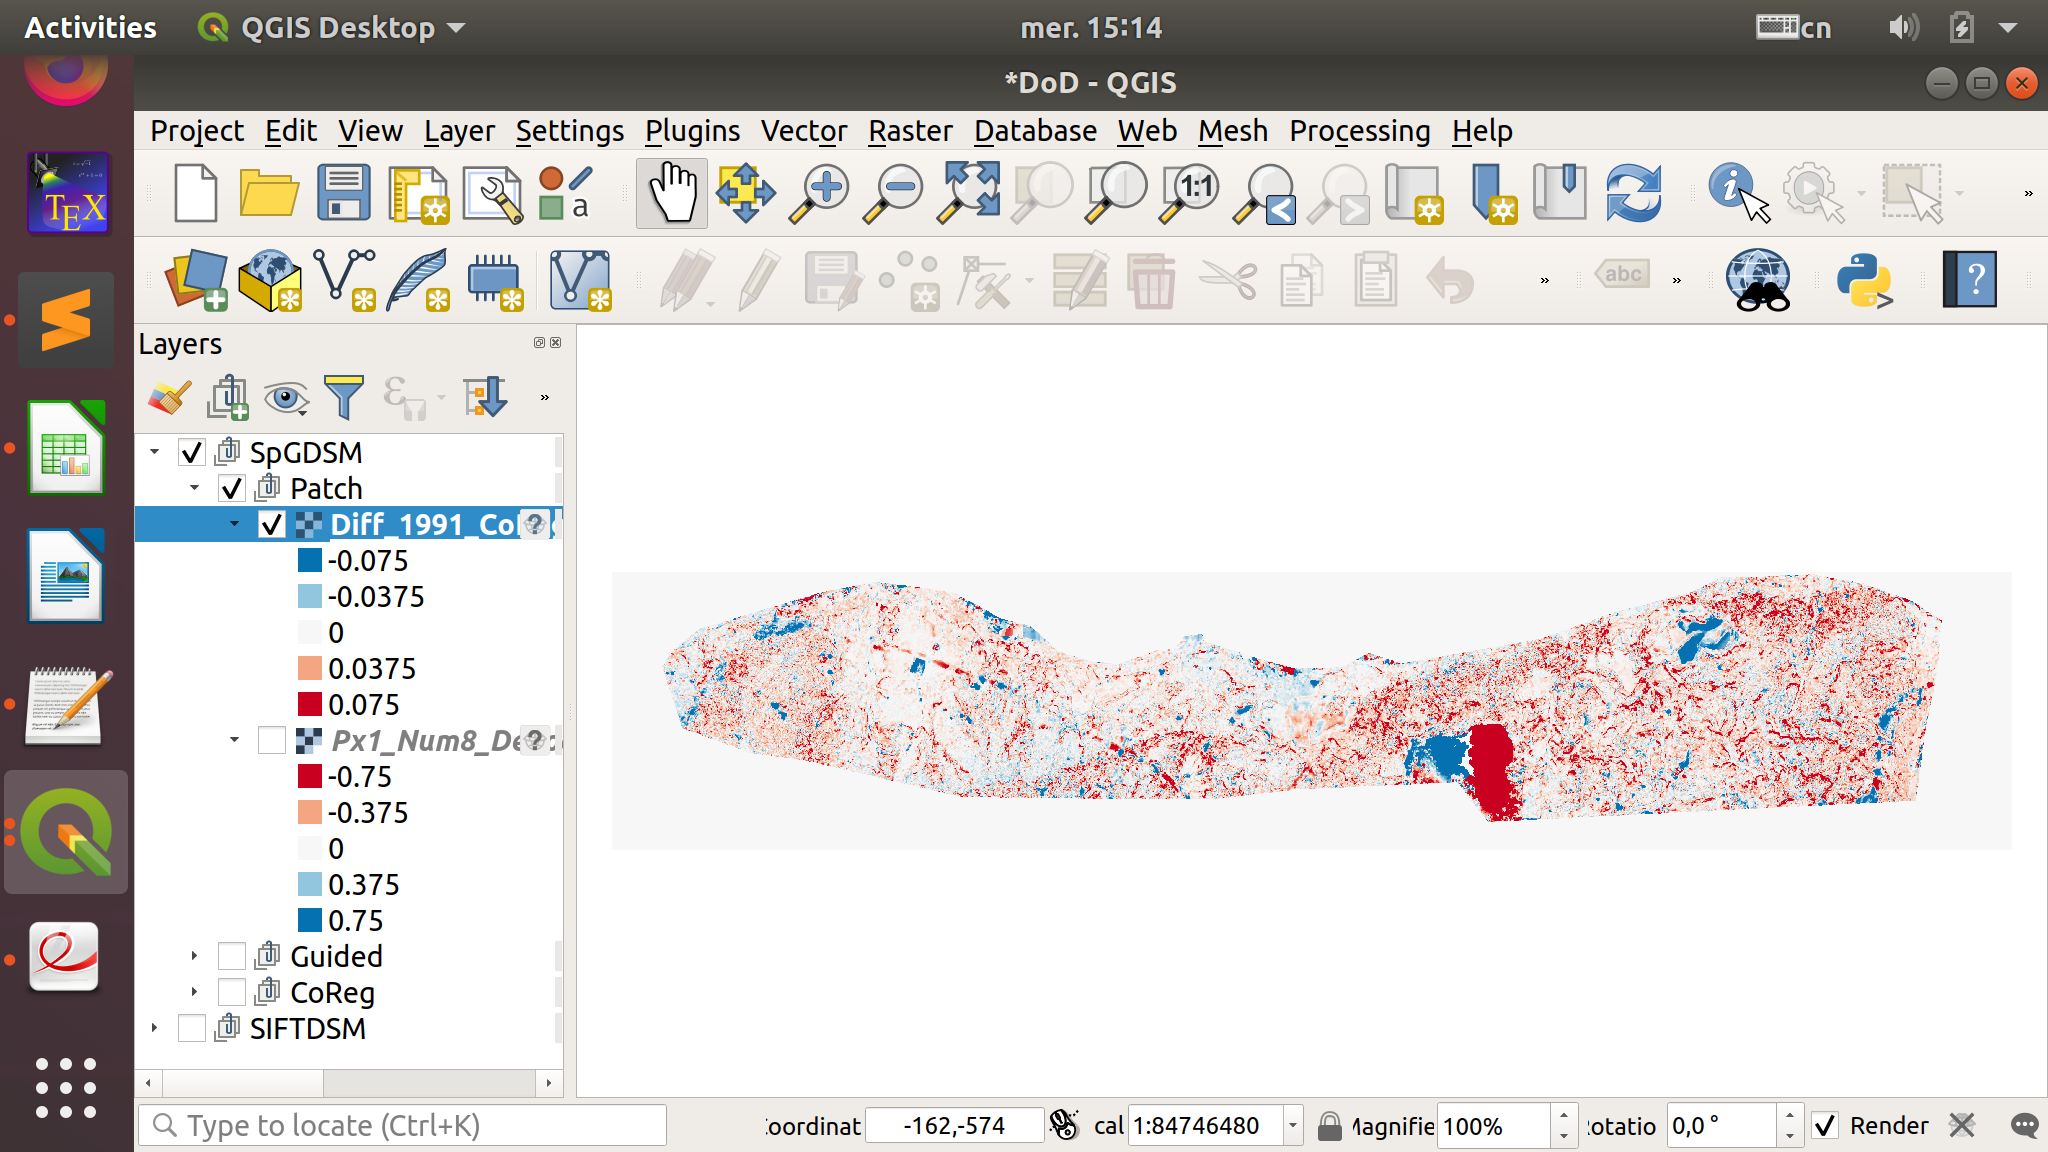
\includegraphics[width=12cm,trim=680 330 100 570,clip]{images/Chapitre4/DoD1991_Patch_SpGDSM.png}
			\end{minipage}%
		}
		\subfigure[\ac{DoD}$_{Kobe}^{Guided_{SpGDSM}}$]{
			\begin{minipage}[t]{1\linewidth}
				\centering
				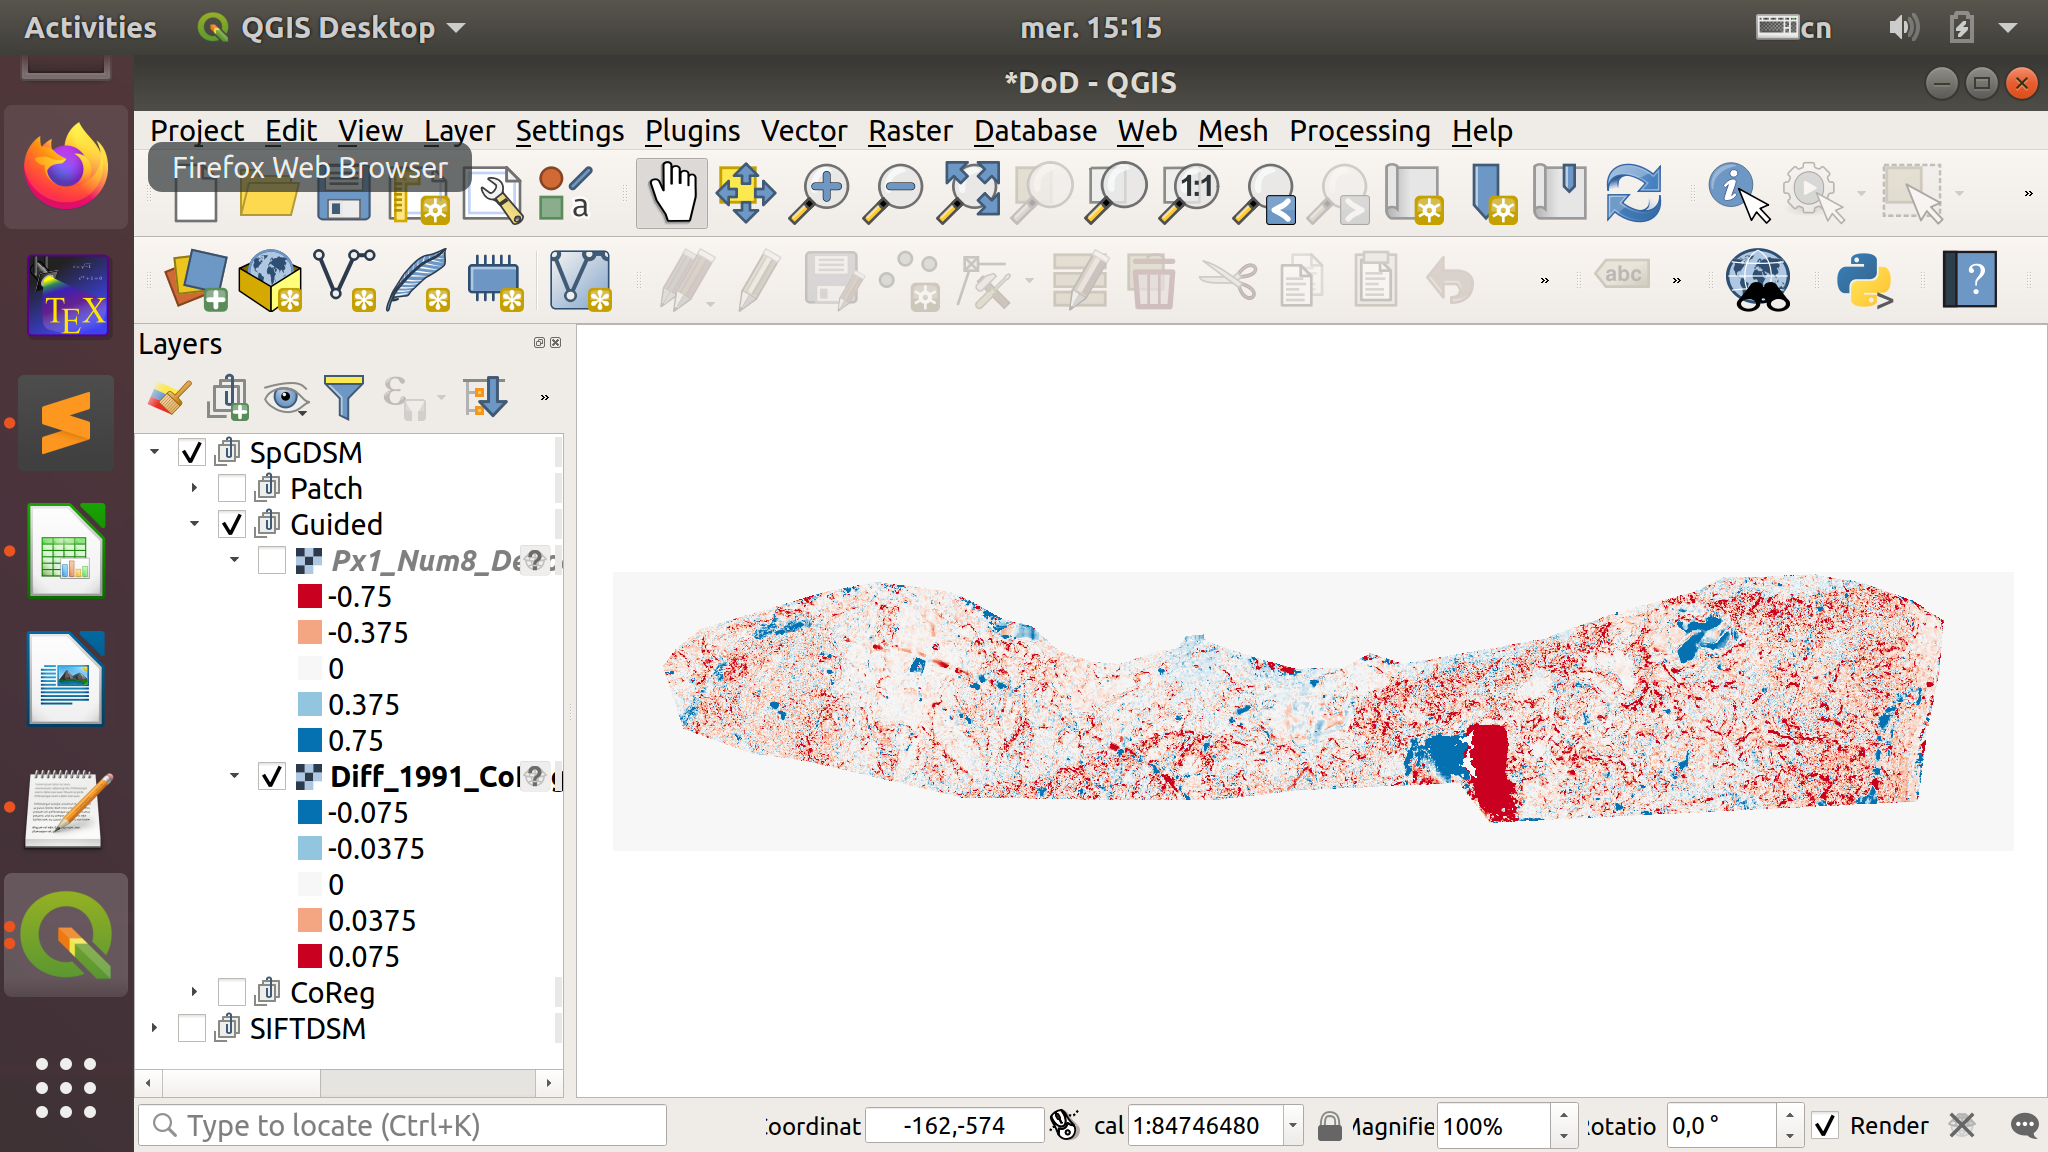
\includegraphics[width=12cm,trim=680 330 100 570,clip]{images/Chapitre4/DoD1991_Guided_SpGDSM.png}
			\end{minipage}%
		}\\
		\subfigure[\ac{DoD}$_{Kobe}^{{SIFTDSM}}$]{
			\begin{minipage}[t]{1\linewidth}
				\centering
				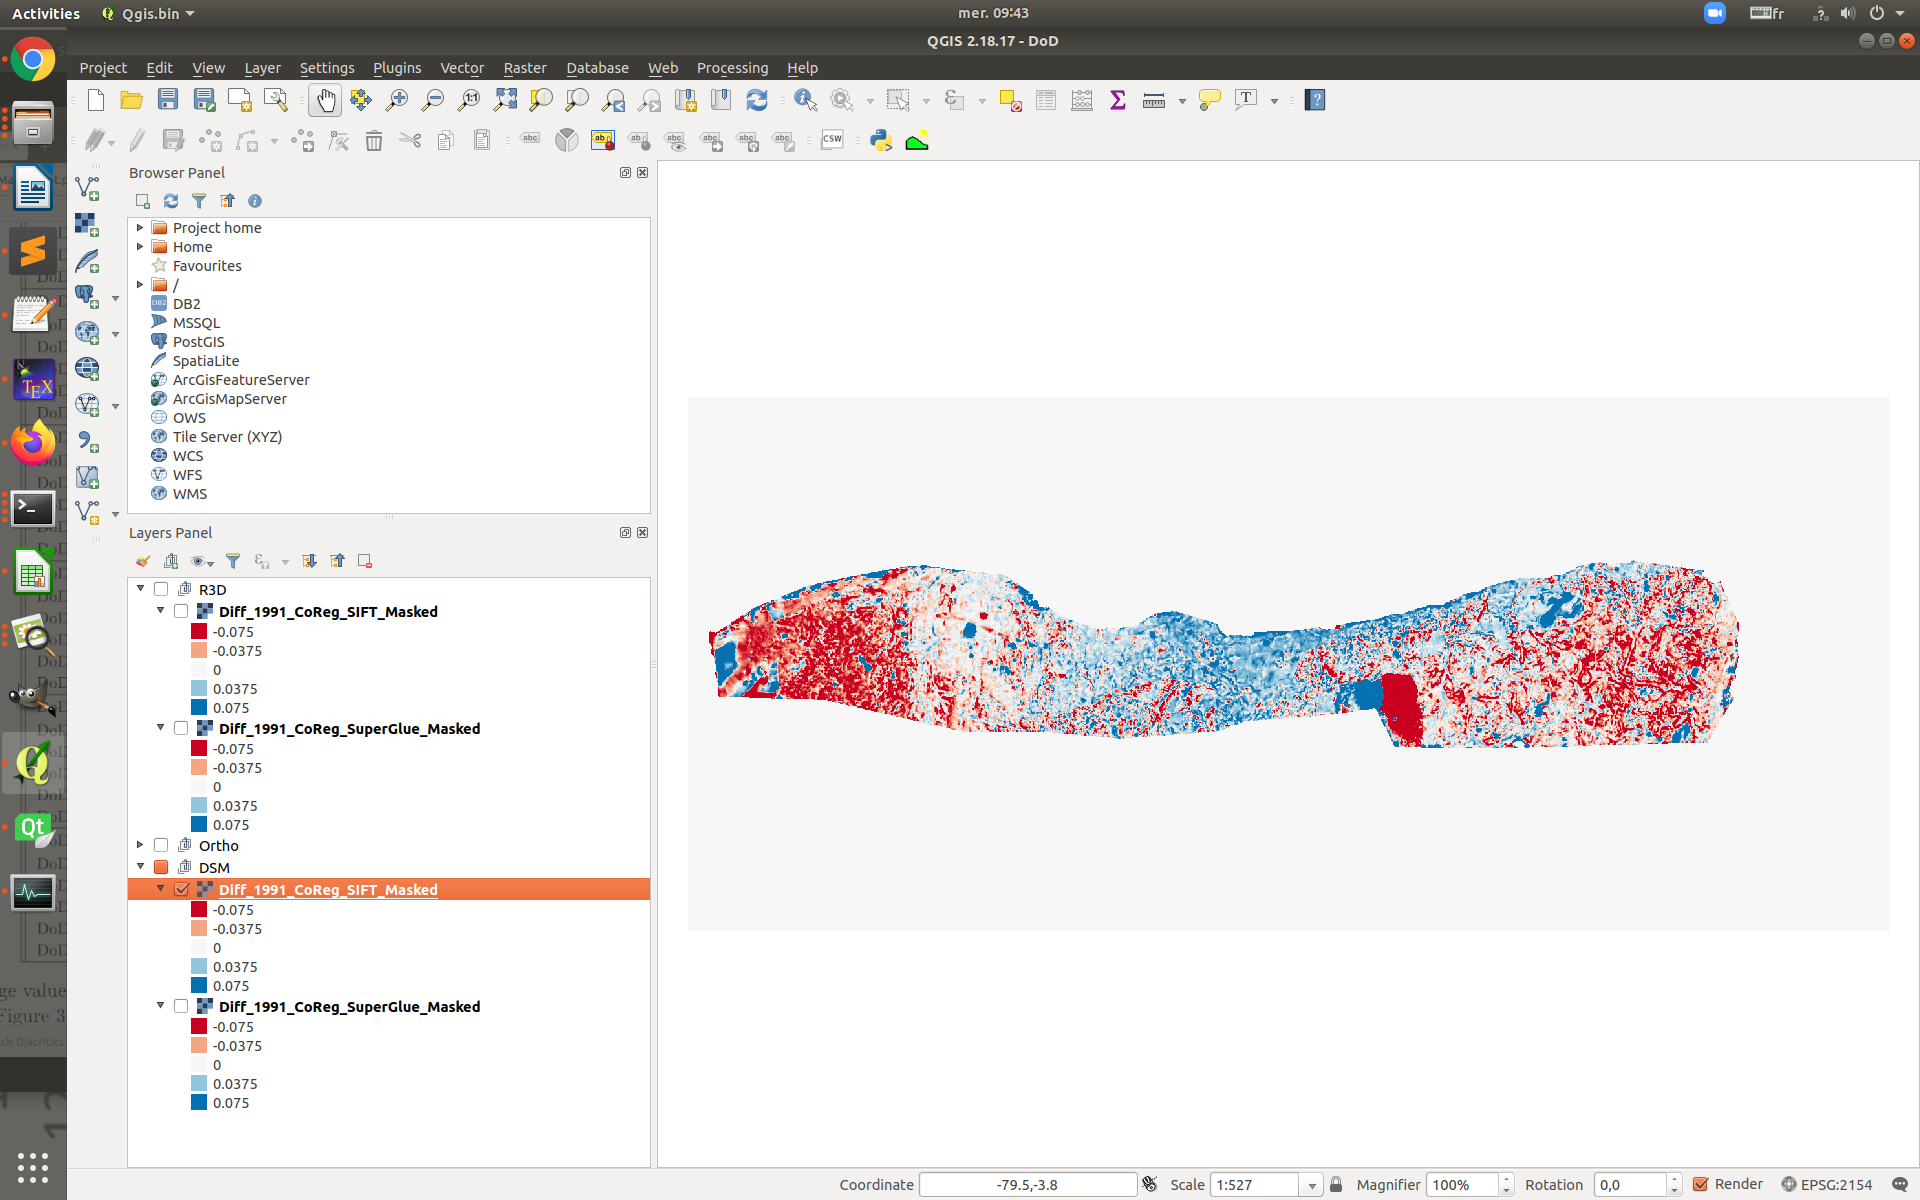
\includegraphics[width=12cm,trim=700 450 180 560,clip]{images/Chapitre3/DoD1991DSM-SIFT.png}
			\end{minipage}%
		}
		\subfigure[\ac{DoD}$_{Kobe}^{Patch_{SIFTDSM}}$]{
			\begin{minipage}[t]{1\linewidth}
				\centering
				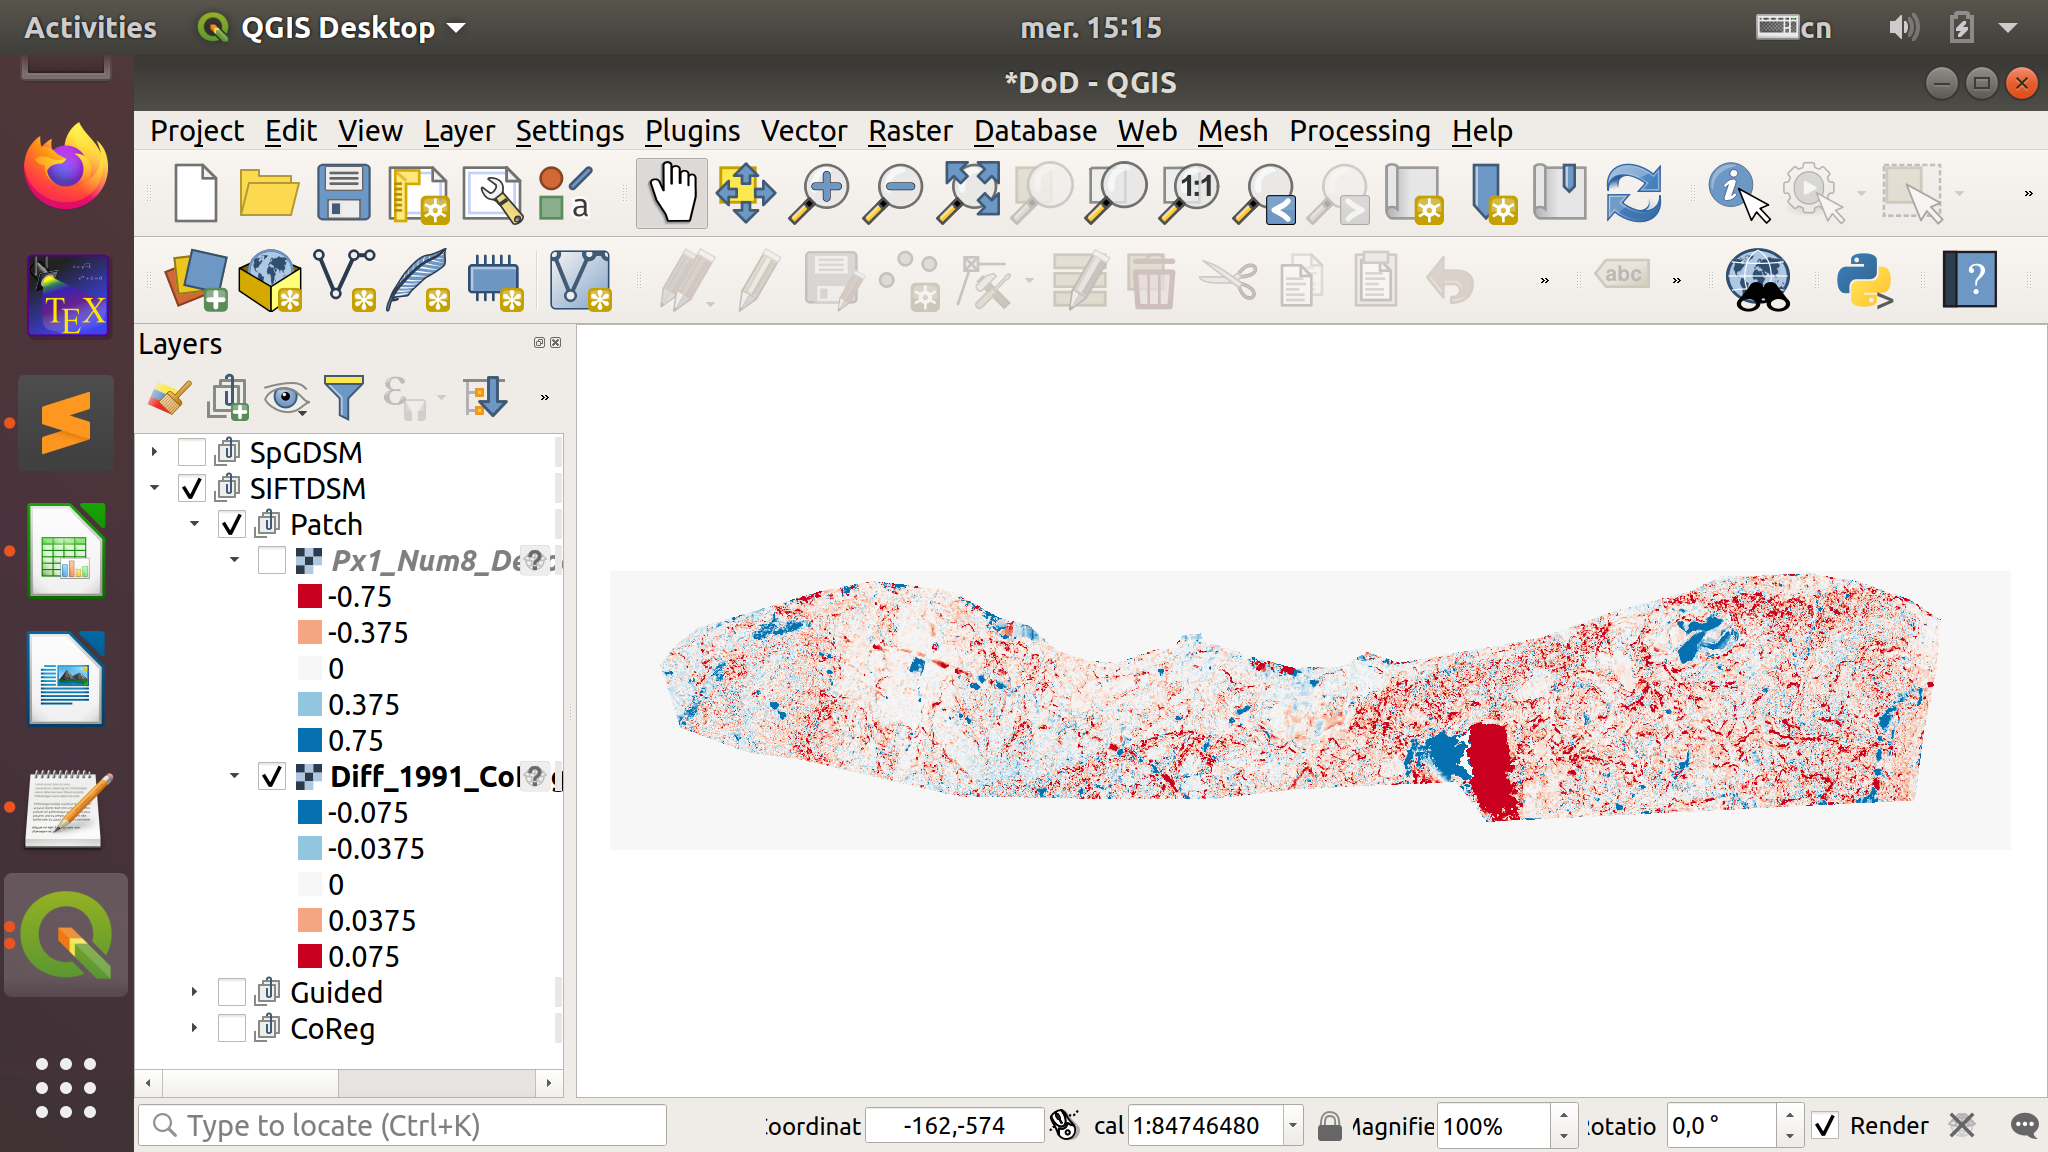
\includegraphics[width=12cm,trim=680 330 100 570,clip]{images/Chapitre4/DoD1991_Patch_SIFTDSM.png}
			\end{minipage}%
		}
		\subfigure[\ac{DoD}$_{Kobe}^{Guided_{SIFTDSM}}$]{
			\begin{minipage}[t]{1\linewidth}
				\centering
				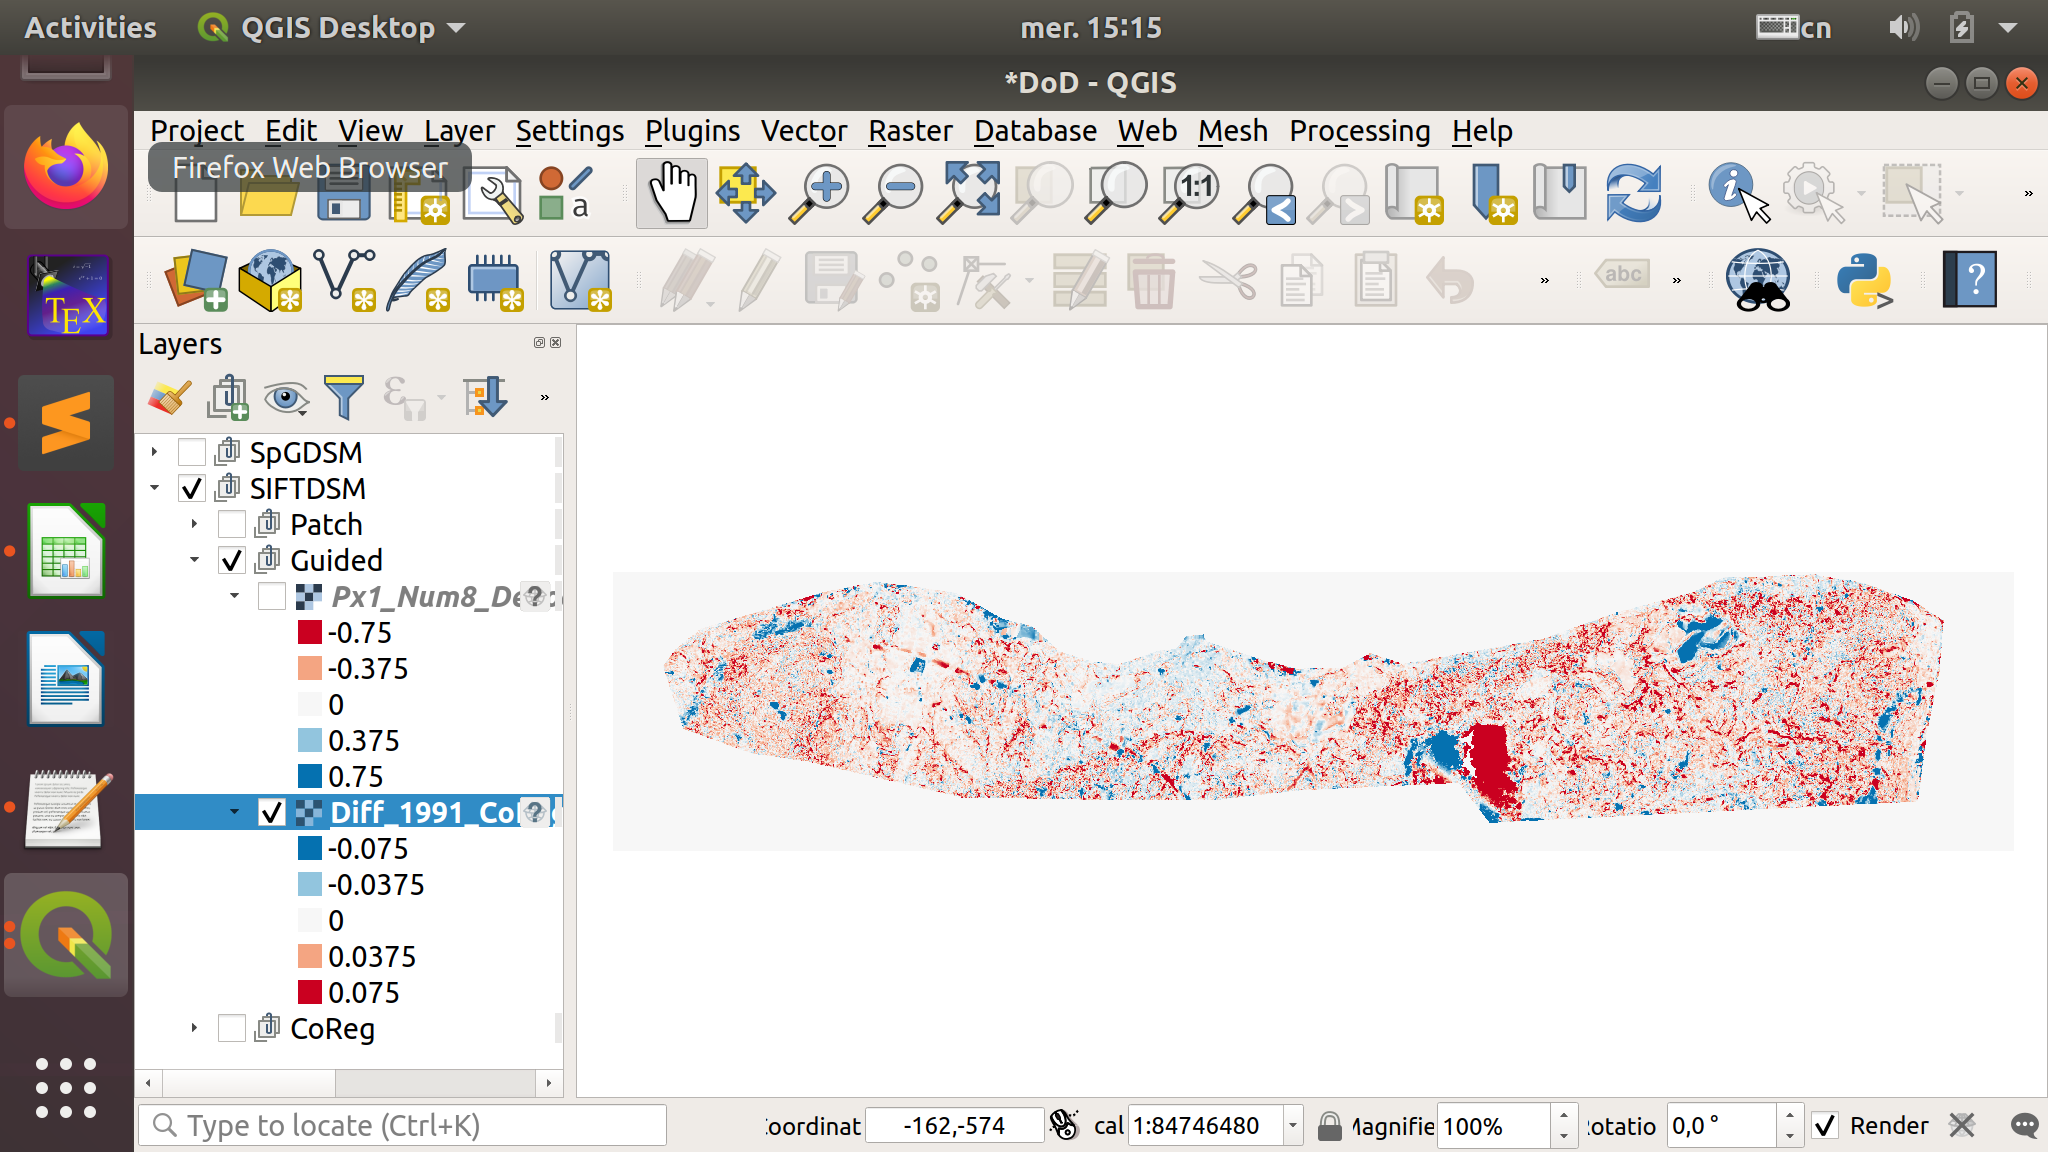
\includegraphics[width=12cm,trim=680 330 100 570,clip]{images/Chapitre4/DoD1991_Guided_SIFTDSM.png}
			\end{minipage}%
		}
		
		\subfigure[\ac{DoD} legend]{
			\begin{minipage}[t]{1\linewidth}
				\centering
				
\includegraphics[width=11cm]{images/Chapitre4/LegendDoD.png}
			\end{minipage}%
		}
		\caption{{\ac{DoD}s between free epoch \textbf{Kobe 1991} and reference epoch \textbf{1995}. (a) and (d) are roughly co-registered \ac{DoD}s resulted from variants $SuperGlue_{DSM}$ and $SIFT_{DSM}$ (elaborated in Chapter~\ref{chap:RoughCoReg}). (b, c, e, f) are refined \ac{DoD}s resulted from variants $Patch_{SpGDSM}$, $Guided_{SpGDSM}$, $Patch_{SIFTDSM}$ and $Guided_{SIFTDSM}$ individually.}}
		\label{PreciseDoDKobe}
	\end{center}
\end{figure*} 



\begin{table}%[H]
	\footnotesize
	\centering
	\begin{tabular}{||l|l|c|c|c||}\hline
		& &$\mu$ [m]&$\sigma$ [m]&$|\mu|$ [m]\\\hline\hline
				%%%%%%%%%%%%%%%%%%%%%%%%satellite
		\multirow{6}{*}{$DoD^{Pezenas}_{1971-2014(Satellite)}$}
		&${{SpGDSM}}$ & -3.70 & 10.65 & 8.29\\
		&${Patch_{SpGDSM}}$ & -0.34 & 4.39 & 2.28\\
		&${Guided_{SpGDSM}}$ & -0.65 & 4.46 & 2.45\\
		&${{SIFTDSM}}$ & -0.68 & 8.11 & 5.80\\
		&${Patch_{SIFTDSM}}$ & -0.49 & 4.41 & 2.29\\
		&${Guided_{SIFTDSM}}$ & -0.57 & 4.38 & \textbf{2.27}\\\hline
		
		\multirow{6}{*}{$DoD^{Kobe}_{1991-1995}$}
		&${{SpGDSM}}$ & -0.75 & 14.62 & 7.95\\
		&${Patch_{SpGDSM}}$ & 1.93 & 10.26 & 3.99\\
		&${Guided_{SpGDSM}}$ & 2.03 & 11.74 & 4.30\\
		&${{SIFTDSM}}$ & 0.27 & 14.40 & 7.57\\
		&${Patch_{SIFTDSM}}$ & 1.80 & 10.36 & 4.00\\
		&${Guided_{SIFTDSM}}$ & 1.84 & 9.48 & \textbf{3.87}\\\hline
				
	\end{tabular}
	\caption{Average value $\mu$, standard deviation $\sigma$, and absolute average value $|\mu|$ of all the \ac{DoD}s in Figure~\ref{PreciseDoDPezenas-Satellite} and ~\ref{PreciseDoDKobe}.}
	\label{PreciseDoDStatistic1}
\end{table}


